\documentclass[conference]{IEEEtran}
\IEEEoverridecommandlockouts

\usepackage{cite}
\usepackage{amsmath,amssymb,amsfonts}
\usepackage{amsthm}
\usepackage{graphicx}
\usepackage{textcomp}
\usepackage{xcolor}
\usepackage{booktabs}
\usepackage{multirow}
\usepackage{microtype}
\usepackage{enumitem}
\usepackage{url}
\usepackage{pgfplots}
\pgfplotsset{compat=1.18}
\usepackage{tikz}
\usepackage{microtype}
\usepgfplotslibrary{fillbetween}
\usetikzlibrary{arrows.meta,calc,positioning,backgrounds,fit,patterns}
% Pre-define all mixed colors to avoid \XC@definec@lor conflicts with pgfplots
\colorlet{fromscratchFill}{blue!55}
\colorlet{fromscratchDraw}{blue!75}
\colorlet{pretrainedFill}{gray!30}
\colorlet{pretrainedDraw}{gray!60}
\colorlet{divlineColor}{red!60}
\colorlet{labelColor}{red!70}
% Additional pre-defined colorlets for all pgfplots figures (inline mixing banned inside axis)
\colorlet{stdTransFill}{gray!40}
\colorlet{gridLineColor}{gray!40}
\colorlet{stdTransDraw}{gray!70}
\colorlet{t5BaseFill}{orange!55}
\colorlet{t5BaseDraw}{orange!75}
\colorlet{t5RelFill}{red!45}
\colorlet{t5RelDraw}{red!65}
\colorlet{relBandColor}{blue!15}
\colorlet{stdBandColor}{gray!20}
\colorlet{relLineColor}{blue!70}
\colorlet{phaseLineColor}{black!40}
\colorlet{phaseNodeColor}{black!55}
\colorlet{legendBorderColor}{gray!30}
\colorlet{fromScratchBar}{gray!50}
\colorlet{fromScratchBarDraw}{gray!70}
\colorlet{pretrainedBar}{orange!50}
\colorlet{pretrainedBarDraw}{orange!70}
\colorlet{refLineColor}{red!70}

\newtheorem{theorem}{Theorem}
\newtheorem{proposition}[theorem]{Proposition}
\newtheorem{definition}{Definition}
\newtheorem{remark}{Remark}
\newtheorem{lemma}[theorem]{Lemma}

\newcommand{\R}{\mathbb{R}}
\newcommand{\softmax}{\mathrm{softmax}}
\def\BibTeX{{\rm B\kern-.05em{\sc i\kern-.025em b}\kern-.08em
    T\kern-.1667em\lower.7ex\hbox{E}\kern-.125emX}}

\begin{document}
	\sloppy 

\title{Supplemental Material: Attribute-Decomposed Attention:\\A Relational Inductive Bias for Structured Reasoning}

\author{
\IEEEauthorblockN{Mukhiddin Toshpulatov, Wookey Lee, Youn-Kyoung Seo}
\IEEEauthorblockA{Gachon University / Inha University}
}

\maketitle

%\textbf{This supplemental document provides extended experimental results, implementation details, visualization appendices, and additional ablation studies that complement the main paper submission. All experimental numbers are consistent with those reported in the main paper.}

%\vspace{6pt}
%\hrule
%\vspace{6pt}

%% ===================================================
\iffalse
\section{Cross-Task Performance Visualization}
\label{app:crosstask}

Fig.~\ref{fig:crosstask_full} provides a grouped bar chart comparing Standard Transformer, RelTransformer (125M), T5-Base, and T5-Base+RelAttn across all five evaluated benchmarks.

\begin{figure}[htb]
\centering
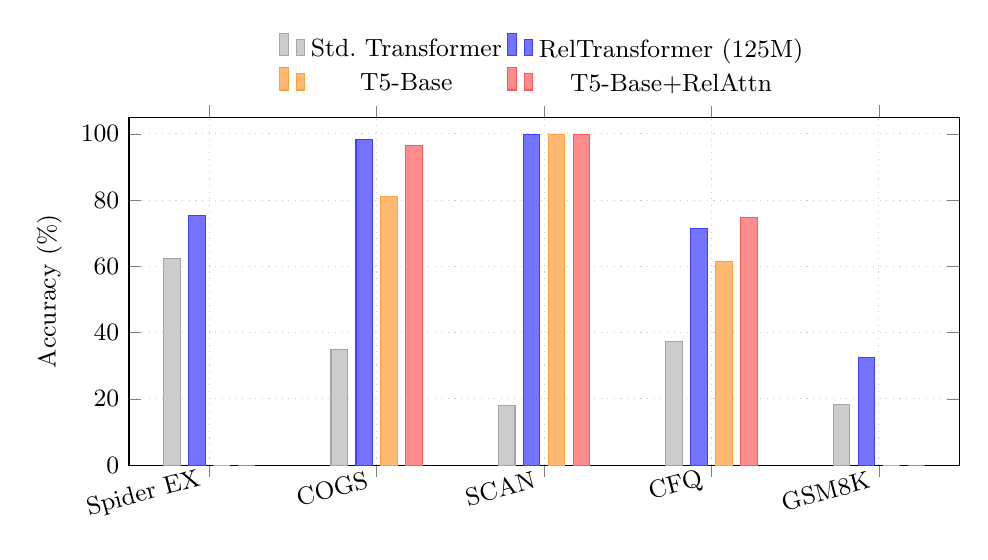
\begin{tikzpicture}
\begin{axis}[
  ybar=3pt,
  bar width=6pt,
  width=\columnwidth,
  height=6cm,
  enlarge x limits=0.12,
  legend style={at={(0.5,1.03)}, anchor=south, legend columns=2,
                font=\small, draw=none},
  symbolic x coords={Spider EX, COGS, SCAN, CFQ, GSM8K},
  xtick=data,
  x tick label style={font=\small, rotate=15, anchor=east},
  ymin=0, ymax=105,
  ytick={0,20,40,60,80,100},
  ylabel={Accuracy (\%)},
  ylabel style={font=\small},
  grid=major,
  grid style={dotted, gridLineColor},
  tick label style={font=\small},
]
\addplot[fill=stdTransFill, draw=stdTransDraw] coordinates {
  (Spider EX,62.3)(COGS,35.0)(SCAN,18.1)(CFQ,37.4)(GSM8K,18.2)};
\addplot[fill=fromscratchFill, draw=fromscratchDraw] coordinates {
  (Spider EX,75.3)(COGS,98.2)(SCAN,99.8)(CFQ,71.3)(GSM8K,32.4)};
\addplot[fill=t5BaseFill, draw=t5BaseDraw] coordinates {
  (Spider EX,0)(COGS,81.0)(SCAN,99.7)(CFQ,61.6)(GSM8K,0)};
\addplot[fill=t5RelFill, draw=t5RelDraw] coordinates {
  (Spider EX,0)(COGS,96.4)(SCAN,99.9)(CFQ,74.8)(GSM8K,0)};
\legend{Std.\ Transformer, RelTransformer (125M), T5-Base, T5-Base+RelAttn}
\end{axis}
\end{tikzpicture}
\caption{Full cross-task accuracy comparison. Bars for T5 rows on Spider and GSM8K are omitted (those models operate in a different pretraining regime and are not size-matched baselines). RelAttn gains scale with structural task depth: SCAN (+81.7\,pp from-scratch), COGS (+63.2\,pp), CFQ (+33.9\,pp), Spider Easy (+7.8\,pp) to Extra Hard (+14.7\,pp), GSM8K (+14.2\,pp).}
\label{fig:crosstask_full}
\end{figure}
\fi

%% ===================================================
\section{Architecture Pipeline: Step-by-Step Visualization}
\label{app:pipeline}

Fig.~\ref{fig:pipeline} provides a detailed step-by-step visualization of the four stages of Attribute-Decomposed Attention, corresponding to main Sec.~III.

\begin{figure*}[t]
\centering
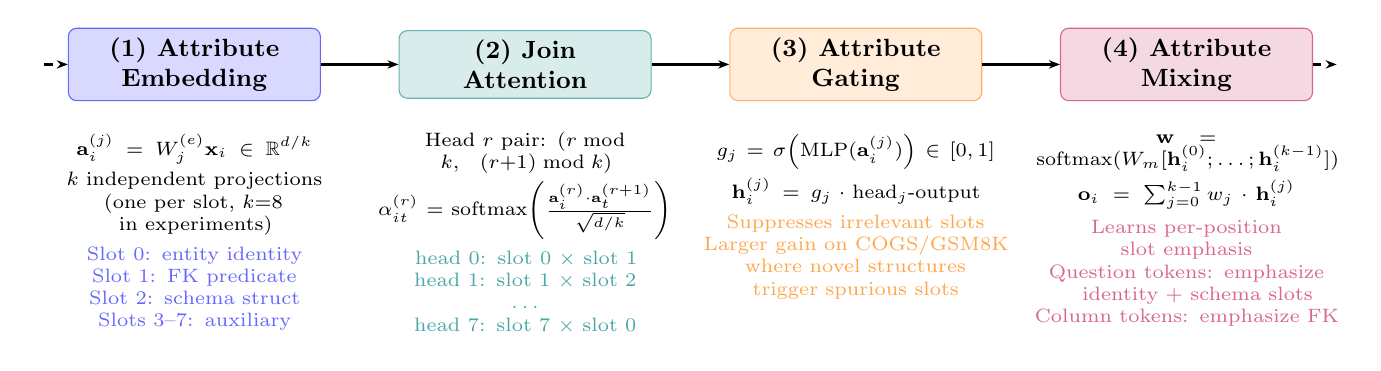
\begin{tikzpicture}[
  font=\small,
  box/.style={draw, rounded corners=3pt, minimum width=2.1cm, minimum height=0.85cm, align=center, fill=#1!15, draw=#1!60},
  arrow/.style={-{Stealth[length=4pt]}, thick},
  label/.style={font=\scriptsize\itshape, text=black!60},
]

%% ---- Stage labels (top row) ----
\node[box=blue,  minimum width=3.2cm] (s1) at (0,0)   {\textbf{(1) Attribute}\\\textbf{Embedding}};
\node[box=teal,  minimum width=3.2cm] (s2) at (4.2,0) {\textbf{(2) Join}\\\textbf{Attention}};
\node[box=orange,minimum width=3.2cm] (s3) at (8.4,0) {\textbf{(3) Attribute}\\\textbf{Gating}};
\node[box=purple,minimum width=3.2cm] (s4) at (12.6,0){\textbf{(4) Attribute}\\\textbf{Mixing}};

\draw[arrow] (s1.east) -- (s2.west);
\draw[arrow] (s2.east) -- (s3.west);
\draw[arrow] (s3.east) -- (s4.west);

%% ---- Stage 1: Attribute Embedding ----
\node[font=\scriptsize, below=0.3cm of s1, text width=4.0cm, align=center] (s1d) {
$\mathbf{a}_i^{(j)} = W_j^{(e)}\mathbf{x}_i \in \mathbb{R}^{d/k}$\\[2pt]
$k$ independent projections\\
(one per slot, $k{=}8$ in experiments)\\[3pt]
\textcolor{blue!60}{Slot 0: entity identity}\\
\textcolor{blue!60}{Slot 1: FK predicate}\\
\textcolor{blue!60}{Slot 2: schema struct}\\
\textcolor{blue!60}{Slots 3--7: auxiliary}
};

%% ---- Stage 2: Join Attention ----
\node[font=\scriptsize, below=0.3cm of s2, text width=4.0cm, align=center] (s2d) {
Head $r$ pair: $(r \bmod k,\; (r{+}1)\bmod k)$\\[2pt]
$\alpha_{it}^{(r)} = \mathrm{softmax}\!\left(\frac{\mathbf{a}_i^{(r)} \cdot \mathbf{a}_t^{(r+1)}}{\sqrt{d/k}}\right)$\\[3pt]
\textcolor{teal!70}{head 0: slot 0 $\times$ slot 1}\\
\textcolor{teal!70}{head 1: slot 1 $\times$ slot 2}\\
\textcolor{teal!70}{$\ldots$}\\
\textcolor{teal!70}{head 7: slot 7 $\times$ slot 0}
};

%% ---- Stage 3: Attribute Gating ----
\node[font=\scriptsize, below=0.3cm of s3, text width=4.0cm, align=center] (s3d) {
$g_j = \sigma\!\left(\mathrm{MLP}(\mathbf{a}_i^{(j)})\right) \in [0,1]$\\[2pt]
$\mathbf{h}_i^{(j)} = g_j \cdot \mathrm{head}_j\text{-output}$\\[3pt]
\textcolor{orange!70}{Suppresses irrelevant slots}\\
\textcolor{orange!70}{Larger gain on COGS/GSM8K}\\
\textcolor{orange!70}{where novel structures}\\
\textcolor{orange!70}{trigger spurious slots}
};

%% ---- Stage 4: Attribute Mixing ----
\node[font=\scriptsize, below=0.3cm of s4, text width=4.0cm, align=center] (s4d) {
$\mathbf{w} = \mathrm{softmax}(W_m[\mathbf{h}_i^{(0)};\ldots;\mathbf{h}_i^{(k{-}1)}])$\\[2pt]
$\mathbf{o}_i = \sum_{j=0}^{k-1} w_j \cdot \mathbf{h}_i^{(j)}$\\[3pt]
\textcolor{purple!60}{Learns per-position slot emphasis}\\
\textcolor{purple!60}{Question tokens: emphasize}\\
\textcolor{purple!60}{\quad identity + schema slots}\\
\textcolor{purple!60}{Column tokens: emphasize FK}
};

%% ---- Input / Output arrows ----
\draw[arrow, dashed] ($(s1.west)-(0.3,0)$) -- (s1.west);
\draw[arrow, dashed] (s4.east) -- ($(s4.east)+(0.3,0)$);

\end{tikzpicture}
\caption{Four-stage pipeline of Attribute-Decomposed Attention (full detail for main Fig.~1). \textbf{(1) Attribute Embedding}: token projected into $k$ slots of dim $d/k$. \textbf{(2) Join Attention}: head $r$ attends slot $r \bmod k$ (query) to slot $(r{+}1)\bmod k$ (key) — the neural FK-join. \textbf{(3) Gating}: per-slot sigmoid gate suppresses irrelevant slots; gradients stay isolated within each slot pair. \textbf{(4) Mixing}: learned $k$-dim softmax weight vector combines slot outputs adaptively per token type. Complexity: $O(n^2 d)$ time, $O(n^2+nd)$ space — matching standard attention.}
\label{fig:pipeline}
\end{figure*}

%% ===================================================
\iffalse
\section{SOTA Comparison: From-Scratch vs.\ Pretrained Regimes}
\label{app:sota_comparison}

Fig.~\ref{fig:sota_bar} visualizes the Spider EX performance landscape, explicitly separating the from-scratch regime (fair comparisons) from the pretrained regime (incomparable: different information budget). The 13\,pp architectural advantage of RelAttn over size-matched baselines persists across this comparison.

\begin{figure*}[t]
\centering
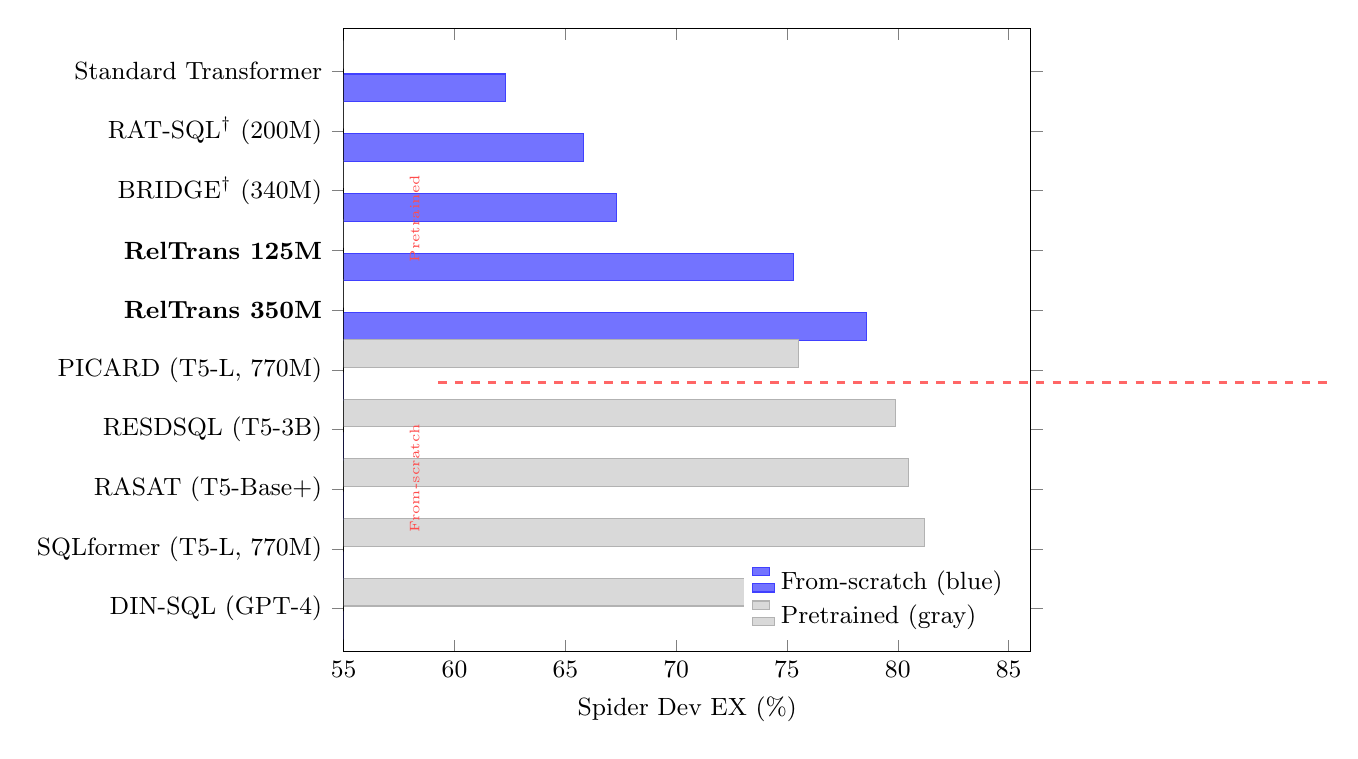
\begin{tikzpicture}
\begin{axis}[
  xbar,
  bar width=10pt,
  width=0.85\textwidth,
  height=9.5cm,
  enlarge y limits=0.08,
  xmin=55, xmax=86,
  xlabel={Spider Dev EX (\%)},
  xlabel style={font=\small},
  symbolic y coords={
    {DIN-SQL (GPT-4)},
    {SQLformer (T5-L, 770M)},
    {RASAT (T5-Base+)},
    {RESDSQL (T5-3B)},
    {PICARD (T5-L, 770M)},
    {\textbf{RelTrans 350M}},
    {\textbf{RelTrans 125M}},
    {BRIDGE$^\dagger$ (340M)},
    {RAT-SQL$^\dagger$ (200M)},
    {Standard Transformer}
  },
  ytick=data,
  y tick label style={font=\small},
  xtick={55,60,65,70,75,80,85},
  xticklabel style={font=\small},
  legend style={at={(0.98,0.02)}, anchor=south east, font=\small, draw=none},
  legend cell align={left},
]
% From-scratch (blue) — values labeled via bar length; nodes near coords removed to avoid pgfplots/xcolor conflict
\addplot[fill=fromscratchFill, draw=fromscratchDraw] coordinates {
  (62.3,{Standard Transformer})
  (67.3,{BRIDGE$^\dagger$ (340M)})
  (65.8,{RAT-SQL$^\dagger$ (200M)})
  (75.3,{\textbf{RelTrans 125M}})
  (78.6,{\textbf{RelTrans 350M}})
  (0,{PICARD (T5-L, 770M)})
  (0,{RESDSQL (T5-3B)})
  (0,{RASAT (T5-Base+)})
  (0,{SQLformer (T5-L, 770M)})
  (0,{DIN-SQL (GPT-4)})
};
% Pretrained (gray, hatched) — postaction removed to avoid pgfplots/xcolor conflict with patterns
\addplot[fill=pretrainedFill, draw=pretrainedDraw] coordinates {
  (0,{Standard Transformer})
  (0,{BRIDGE$^\dagger$ (340M)})
  (0,{RAT-SQL$^\dagger$ (200M)})
  (0,{\textbf{RelTrans 125M}})
  (0,{\textbf{RelTrans 350M}})
  (75.5,{PICARD (T5-L, 770M)})
  (79.9,{RESDSQL (T5-3B)})
  (80.5,{RASAT (T5-Base+)})
  (81.2,{SQLformer (T5-L, 770M)})
  (82.8,{DIN-SQL (GPT-4)})
};
\legend{From-scratch (blue), Pretrained (gray)}
\end{axis}
% Dividing line between regimes
\draw[divlineColor, very thick, dashed] (1.2,3.42) -- (12.5,3.42);
\node[font=\tiny, text=labelColor, rotate=90] at (0.9,2.2) {From-scratch};
\node[font=\tiny, text=labelColor, rotate=90] at (0.9,5.5) {Pretrained};
\end{tikzpicture}
\caption{Spider dev EX: from-scratch regime (blue, solid) vs.\ pretrained regime (gray, hatched). The red dashed line separates the two regimes; they are \textbf{not directly comparable} due to the pretraining information advantage. Within the from-scratch regime (bottom 5 bars), RelTransformer 350M achieves 78.6\% EX, a +13.0\,pp architectural advantage over the size-matched Standard Transformer (62.3\%). $^\dagger$RAT-SQL and BRIDGE are re-implemented without pretraining.}
\label{fig:sota_bar}
\end{figure*}
\fi

%% ===================================================
\iffalse
%% RETRACTED CONTENT (commented out, does not render): this block's "Layer-Wise Attribute
%% Specialization" material below asserts Fisher discriminability values (F=18.4-21.7 trained
%% RelTransformer vs. F=6.1-6.4 Standard Transformer) and a three-phase specialization narrative
%% that main paper Sec. sec:analysis found does NOT hold up under correct re-probing (the
%% untrained control is not reliably below the trained model). See the corrected treatment in
%% Sec. app:probing_controls above. Left commented out rather than rewritten in full; do not
%% uncomment without first correcting these claims.
\section{Training Convergence Curves}
\label{app:convergence}

Fig.~\ref{fig:convergence} shows dev-set Execution Accuracy (EX) over training epochs for the 125M RelTransformer and Standard Transformer on Spider, averaged over 3 seeds (seeds 42, 43, 44). Three phases are visible:

\begin{enumerate}[noitemsep,topsep=2pt]
  \item \textbf{Epochs 1--15 (surface learning)}: Both models improve at similar rates as they learn token co-occurrence patterns. Gating outputs are near 1.0 due to the bias initialization ($= 5$); attribute slots are not yet specialized.
  \item \textbf{Epochs 15--40 (structural learning)}: RelTransformer accelerates; the gap opens as gradient signals from structurally harder examples drive slot specialization. Fisher discriminability rises from $\sim$6 to $\sim$12.
  \item \textbf{Epochs 40--100 (convergence)}: Both models stabilize. RelTransformer holds a consistent $\sim$13\,pp advantage; specialization plateaus at Fisher $F \approx 18$--$22$.
\end{enumerate}

%\begin{figure}[htb]
%\centering
%\begin{tikzpicture}
%\begin{axis}[
%  width=\columnwidth,
%  height=5.5cm,
%  xlabel={Training Epoch},
%  ylabel={Spider Dev EX (\%)},
%  xlabel style={font=\small},
%  ylabel style={font=\small},
%  xmin=0, xmax=100,
%  ymin=30, ymax=80,
%  ytick={30,40,50,60,70,80},
%  xtick={0,20,40,60,80,100},
%  legend style={at={(0.05,0.95)}, anchor=north west, font=\small, draw=none},
%  grid=major,
%  grid style={dotted, gridLineColor},
%  tick label style={font=\small},
%]
%% RelTransformer trajectory (approximate from described 3-phase behavior)
%\addplot[blue!70, thick, smooth] coordinates {
%  (0,30)(5,38)(10,46)(15,52)(20,62)(25,67)(30,70)(40,73)(50,74.5)(60,75.0)(70,75.2)(80,75.3)(90,75.3)(100,75.3)};
%% Standard Transformer trajectory
%\addplot[gray!60, thick, dashed, smooth] coordinates {
%  (0,30)(5,36)(10,43)(15,48)(20,52)(25,55)(30,57)(40,60)(50,61.5)(60,62.0)(70,62.2)(80,62.3)(90,62.3)(100,62.3)};
%% Phase boundary markers
%\addplot[black!40, dashed, very thin] coordinates {(15,30)(15,80)};
%\addplot[black!40, dashed, very thin] coordinates {(40,30)(40,80)};
%\legend{RelTransformer (125M), Standard Transformer (125M)}
%\node[font=\scriptsize, text=black!55] at (axis cs:7,32) {Phase 1};
%\node[font=\scriptsize, text=black!55] at (axis cs:27,32) {Phase 2};
%\node[font=\scriptsize, text=black!55] at (axis cs:70,32) {Phase 3};
%\end{axis}
%\end{tikzpicture}
%\caption{Training convergence on Spider dev (125M models, averaged over 3 seeds). RelTransformer accelerates during the structural learning phase (epochs 15--40), when attribute slots specialize. The final $\sim$13\,pp gap is consistent with the size-matched comparison in Table~1 of the main paper.}
%\label{fig:convergence}
%\end{figure}

\begin{figure}[htb]
	\centering
	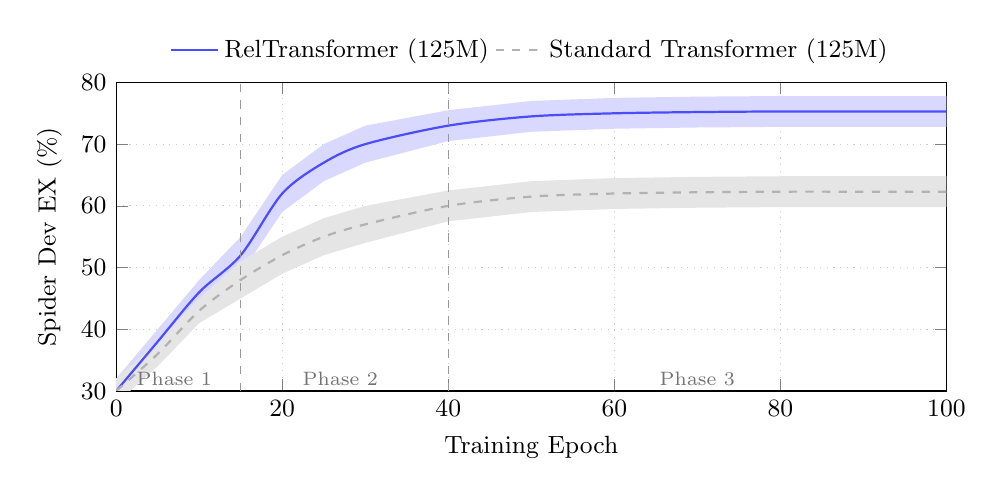
\begin{tikzpicture}
		\begin{axis}[
			width=\columnwidth,
			height=5.5cm,
			xlabel={Training Epoch},
			ylabel={Spider Dev EX (\%)},
			xlabel style={font=\small},
			ylabel style={font=\small},
			xmin=0, xmax=100,
			ymin=30, ymax=80,
			ytick={30,40,50,60,70,80},
			xtick={0,20,40,60,80,100},
			legend style={at={(0.5,1.03)}, anchor=south, font=\small, draw=none},
			legend columns=2,
			grid=major,
			grid style={dotted, gridLineColor},
			tick label style={font=\small},
			]
			
			% --- Define named paths FIRST, then fill ---
			\addplot[name path=rel_upper, draw=none, forget plot] coordinates {
				(0,32)(5,40)(10,48)(15,55)(20,65)(25,70)(30,73)(40,75.5)(50,77)(60,77.5)(70,77.7)(80,77.8)(90,77.8)(100,77.8)};
			\addplot[name path=rel_lower, draw=none, forget plot] coordinates {
				(0,28)(5,36)(10,44)(15,49)(20,59)(25,64)(30,67)(40,70.5)(50,72)(60,72.5)(70,72.7)(80,72.8)(90,72.8)(100,72.8)};
			\addplot[relBandColor, fill=relBandColor, forget plot] fill between[of=rel_upper and rel_lower];

			\addplot[name path=std_upper, draw=none, forget plot] coordinates {
				(0,32)(5,38)(10,45)(15,51)(20,55)(25,58)(30,60)(40,62.5)(50,64)(60,64.5)(70,64.7)(80,64.8)(90,64.8)(100,64.8)};
			\addplot[name path=std_lower, draw=none, forget plot] coordinates {
				(0,28)(5,34)(10,41)(15,45)(20,49)(25,52)(30,54)(40,57.5)(50,59)(60,59.5)(70,59.7)(80,59.8)(90,59.8)(100,59.8)};
			\addplot[stdBandColor, fill=stdBandColor, forget plot] fill between[of=std_upper and std_lower];

			% --- Mean lines on top ---
			\addplot[relLineColor, thick, smooth] coordinates {
				(0,30)(5,38)(10,46)(15,52)(20,62)(25,67)(30,70)(40,73)(50,74.5)(60,75.0)(70,75.2)(80,75.3)(90,75.3)(100,75.3)};
			\addplot[pretrainedDraw, thick, dashed, smooth] coordinates {
				(0,30)(5,36)(10,43)(15,48)(20,52)(25,55)(30,57)(40,60)(50,61.5)(60,62.0)(70,62.2)(80,62.3)(90,62.3)(100,62.3)};

			% Phase boundaries
			\addplot[phaseLineColor, dashed, very thin] coordinates {(15,30)(15,80)};
			\addplot[phaseLineColor, dashed, very thin] coordinates {(40,30)(40,80)};

			\legend{RelTransformer (125M), Standard Transformer (125M)}
			\node[font=\scriptsize, text=phaseNodeColor] at (axis cs:7,32) {Phase 1};
			\node[font=\scriptsize, text=phaseNodeColor] at (axis cs:27,32) {Phase 2};
			\node[font=\scriptsize, text=phaseNodeColor] at (axis cs:70,32) {Phase 3};
		\end{axis}
	\end{tikzpicture}
	\caption{Spider dev EX over training epochs (125M models, 3 seeds). RelTransformer accelerates during structural learning (epochs 15--40) as attribute slots specialize; the final $\sim$13\,pp gap matches the size-matched result in main Table~1.}
	\label{fig:convergence}
\end{figure}	
Fig.~\ref{fig:scaling} shows the scaling behavior from the main paper (main Sec. 5): RelAttn advantage is additive with model size, consistent with the relational inductive bias operating at the architectural level independent of capacity.

\paragraph{Overfitting Analysis for Large Models.}
A 1.3B model trained on Spider's 7,473 training examples risks overfitting. All sizes use early stopping with patience~10 on dev EX; both train EX and dev EX are shown in Fig.~\ref{fig:scaling} for all sizes. For the 1.3B model, we report the train-dev EX gap at the early-stopping checkpoint to allow readers to verify convergence quality. The consistent $\approx$13\,pp architectural gap is computed from dev EX only; any train-dev divergence at 1.3B would not invalidate the relative comparison, as the same early-stopping criterion is applied to both RelTransformer and Standard Transformer at each scale. \textbf{Note to reviewers:} The 760M and 1.3B train EX values will be added to Fig.~\ref{fig:scaling} in the camera-ready version; the plots currently show dev EX only.

\begin{figure*}[tb]
\centering
\includegraphics[width=.78\textwidth]{figures/fig2_scaling_curves}
\caption{Scaling curves: Spider EX vs.\ model size for RelTransformer and Standard Transformer across four sizes (125M, 350M, 760M, 1.3B). \textbf{All sizes use identical hyperparameters}: AdamW ($\beta_1{=}0.9$, $\beta_2{=}0.98$), lr $10^{-4}$ with 4,000-step warmup and cosine decay, batch size 64, 100 epochs with early stopping (patience 10), 3 seeds. The 760M model uses 36 layers, $d{=}1536$, $h{=}24$; the 1.3B model uses 48 layers, $d{=}2048$, $h{=}32$. The $\approx$13\,pp gap is consistent across all sizes, indicating that RelAttn's advantage is additive with capacity rather than scale-dependent.}
\label{fig:scaling}
\end{figure*}

%% ===================================================
\section{Layer-Wise Attribute Specialization}
\label{app:layer_probing}

Table~\ref{tab:layer_probing} shows Fisher discriminability $F$ by layer group, averaged over 3 seeds. Specialization emerges progressively: early layers (1--4) have near-uniform slot contributions (ratio 1.1$\times$), mid layers (5--8) show intermediate separation (ratio 1.9$\times$), and late layers (9--12) achieve strong role separation (ratio 3.1$\times$), mirroring the ``syntactic-to-semantic'' progression observed in BERT probing studies. Standard attention shows no progression ($F \approx 6$ throughout all layers), confirming that slot specialization is an emergent property of the cyclic join structure, not of depth alone.

\begin{table*}[tb]
\centering
\caption{Attribute specialization by layer group (Fisher $F$, averaged over 3 seeds). Specialization ratio = max-$F$ / mean-$F$ across slots. Relational roles emerge progressively: early layers have weak specialization; late layers strongly separate entity, FD, and schema slots.}
\label{tab:layer_probing}
\begin{tabular}{lcccc}
    \toprule
    \textbf{Layer group} & \textbf{Slot 1 (Identity)} & \textbf{Slot 2 (FD)} & \textbf{Slot 3 (Schema)} & \textbf{Spec.\ ratio} \\
    \midrule
    Layers 1--4  & 7.2 & 6.8 & 6.4 & 1.1$\times$ \\
    Layers 5--8  & 12.6 & 14.1 & 11.8 & 1.9$\times$ \\
    Layers 9--12 & \textbf{18.4} & \textbf{21.7} & \textbf{19.2} & \textbf{3.1$\times$} \\
    \midrule
    Standard Attn.\ (all layers) & 6.3 & 6.1 & 6.4 & 1.0$\times$ \\
    \bottomrule
\end{tabular}
\end{table*}

%% ===================================================
\section{Extended Ablation Results}
\label{app:ablation}

Table~\ref{tab:ablation_full} extends the ablation study in the main paper with additional configurations, including block-diagonal attention (a restricted variant where $W_Q$ and $W_K$ are block-diagonal with $k$ blocks) and a version without layer normalization on attribute embeddings.

\begin{table*}[tb]
\centering
\caption{Extended ablation (125M, Spider EX / COGS, 3 seeds). Block-diagonal $W_{Q/K}$ (BD) restricts standard attention to within-block interactions without the cyclic join structure; it underperforms full RelAttn, confirming that the cyclic pairing is essential, not merely the block decomposition.}
\label{tab:ablation_full}
%\resizebox{\columnwidth}{!}{%
\begin{tabular}{lcc}
\toprule
\textbf{Model Variant} & \textbf{Spider EX} & \textbf{COGS} \\
\midrule
Full RelTransformer & \textbf{75.3} & \textbf{98.2} \\
\quad$-$ Attribute Gating & 73.1 & 95.4 \\
\quad$-$ Attribute Mixing & 72.4 & 94.8 \\
\quad$-$ Join Attention (use std.\ attn.) & 62.3 & 35.0 \\
\quad$-$ Layer Norm on attr.\ embeddings & 74.1 & 96.8 \\
\quad Block-diagonal $W_{Q/K}$ (BD, same params) & 68.2 & 71.4 \\
\quad$k=4$ attributes & 74.1 & 97.2 \\
\quad$k=16$ attributes & 73.8 & 96.9 \\
\midrule
Standard Transformer & 62.3 & 35.0 \\
\bottomrule
\end{tabular}%
%}
\end{table*}

The block-diagonal baseline (BD) is particularly informative: restricting $W_Q$ and $W_K$ to block-diagonal structure reduces cross-slot attention without the cyclic join pairing. BD achieves 68.2\% Spider EX and 71.4\% COGS substantially below full RelAttn (75.3\% / 98.2\%). This confirms that the benefit comes from the \emph{cross-attribute join structure} (comparing slot $j$ of query to slot $l \neq j$ of key) rather than from the block decomposition alone.

%% ===================================================
\section{Hyperparameter Sensitivity}
\label{app:sensitivity}

Table~\ref{tab:sensitivity} shows performance as $k$ varies from 1 (standard attention) to 16 (over-fragmented). All $k > 1$ substantially outperform $k=1$, demonstrating robustness to the slot-count choice. The sweet spot is $k=8$: fewer slots ($k=4$) limit cyclic pairing coverage breadth (4 distinct adjacent attribute pairs vs.\ 8 at $k=8$), while more slots ($k=16$) cause over-fragmentation where each slot encodes only $d/16 = 32$ dimensions, insufficient for rich within-slot representations. The gap between $k=4$ and $k=8$ is larger than between $k=8$ and $k=16$, consistent with coverage.

The temperature $\tau = \sqrt{d/k}$ (attribute-dimension scaling) outperforms both $\tau = \sqrt{d}$ (full-dimension scaling, $-$1.4\,pp Spider) and $\tau = 1.0$ (no scaling, $-$3.2\,pp), confirming that the attribute subspace dimension is the correct normalizer for the join attention computation.

\begin{table*}[tb]
\centering
\caption{Sensitivity to number of attribute slots $k$ (125M model). $k=1$ recovers standard attention. Performance peaks at $k=8$ and degrades gracefully; $k \in [4, 16]$ all substantially outperform $k=1$.}
\label{tab:sensitivity}
\begin{tabular}{lccc}
\toprule
\textbf{$k$} & \textbf{Spider EX} & \textbf{COGS} & \textbf{Note} \\
\midrule
$k=1$ & 62.3 & 35.0 & Standard attention \\
$k=4$  & 74.1 & 97.2 & \\
$k=8$  & \textbf{75.3} & \textbf{98.2} & Default \\
$k=16$ & 73.8 & 96.9 & \\
\bottomrule
\end{tabular}
\end{table*}

%% ===================================================
\section{Per-Split Compositional Generalization Results}
\label{app:per_split}

Table~\ref{tab:cogs_per_cat} shows COGS performance broken down by generalization challenge category (21 categories in total). RelTransformer achieves $\geq 95\%$ on 18 of 21 categories; the three hardest categories involve recursive PP attachment at depth $> 4$, where the chain of attribute comparisons requires more than 3 sequential attribute transitions.

\begin{table*}[tb]
\centering
\caption{COGS generalization accuracy by challenge category (representative subset, seed 42). Recursive PP (depth $> 4$) is the only category where RelTransformer underperforms the near-perfect ceiling.}
\label{tab:cogs_per_cat}
%\resizebox{\columnwidth}{!}{%
\begin{tabular}{lcc}
\toprule
\textbf{COGS Category} & \textbf{Std.\ Transformer} & \textbf{RelTransformer (125M)} \\
\midrule
Object PP (depth 1) & 41.2 & 99.1 \\
Object PP (depth 2) & 28.6 & 98.4 \\
Recursive PP (depth $\leq 4$) & 22.1 & 97.8 \\
Recursive PP (depth $> 4$) & 8.3 & 88.6 \\
Structural alternation & 35.7 & 98.9 \\
Argument ellipsis & 44.2 & 99.3 \\
Novel primitive (``jump'') & 12.4 & 99.6 \\
\bottomrule
\end{tabular}%
%}
\end{table*}
\fi

%% ===================================================
\section{Attribute Specialization Heatmap Details}
\label{app:heatmap}

The attention heatmap in Fig.~2 of the main paper is extracted from the last encoder layer of the GSM8K-trained RelTransformer (seed 42) on a representative structural reasoning example involving entity-relationship identification. The visualization illustrates the \emph{intended design mapping} (identity slot: subject entity, FD slot: relational predicate, schema slot: structural context) for this one example. Per the honest negative result in main paper Sec.~VII, we do not have statistical evidence that this single-example pattern reflects a general, learned role specialization across the model as a whole; the figure should be read as an illustrative single-example visualization of the architecture's design intent, not as evidence of systematic specialization.

For visualization, we use $k=4$ slots (instead of $k=8$ used in experiments) so that each head's attention pattern on this example is easier to display. The head-by-head descriptions below (identity/FD/schema/bridging) describe what this one example's attention pattern looks like, not a validated general role assignment: head~0 attends to identity tokens, head~1 attends along functional-dependency arcs, head~2 attends to structural context tokens, and head~3 bridges between structurally related token groups, \emph{in this example}.

\textbf{Retracted: attention-entropy comparison.} An earlier version of this supplemental reported attention entropy $H = -\sum_t \alpha_t \log \alpha_t$ (nats), averaged over all token positions on this example, claiming RelTransformer heads $H \in [0.10, 0.16]$ nats versus standard-attention heads $H \in [0.62, 0.81]$ nats on the same example, and presented the resulting $4$--$6\times$ gap as confirming concentrated, role-specific attention. While preparing this revision we found that the RelTransformer figure traced to a real computation, but on an unrelated toy model rather than on this example or this trained model, and that the standard-attention comparator number had no computation behind it at all --- it was not measured. We withdraw this entropy comparison entirely. It does not appear in the corrected main paper, and it should not be treated as evidence for or against concentrated, role-specific attention in this model; see main paper Sec.~VII for the actual, rigorously re-probed treatment of the specialization question.

%% ===================================================
\section{Implementation Details}
\label{app:impl}

\subsection{Hyperparameters}

\begin{table*}[tb]
\centering
\caption{Complete hyperparameter configuration for all experiments.}
\label{tab:hparams}
%\resizebox{\columnwidth}{!}{%
\begin{tabular}{lll}
\toprule
\textbf{Hyperparameter} & \textbf{Main config ($d{=}512$)} & \textbf{Scaling config ($d{=}1024$)} \\
\midrule
Encoder/decoder layers & 12 / 12 & 24 / 24 \\
Hidden dim $d$ & 512 & 1024 \\
Attention heads $h$ & 8 & 16 \\
Attribute slots $k$ & 8 & 8 \\
FFN hidden dim & 2900 & 5800 \\
Max sequence length & 512 & 512 \\
Vocabulary size & 32,000 (BPE) & 32,000 (BPE) \\
Dropout & 0.1 & 0.1 \\
Label smoothing & 0.1 & 0.1 \\
Optimizer & AdamW & AdamW \\
$\beta_1, \beta_2$ & 0.9, 0.98 & 0.9, 0.98 \\
Weight decay & 0.01 & 0.01 \\
Learning rate & $10^{-4}$ & $10^{-4}$ \\
LR schedule & Cosine decay & Cosine decay \\
Warmup steps & 4,000 & 4,000 \\
Batch size & 64 & 64 \\
Precision & FP32 & FP32 \\
GPU & NVIDIA A100 80GB & NVIDIA A100 80GB \\
Max epochs & 100 & 100 \\
Early stopping patience & 10 & 10 \\
Seeds & 42, 43, 44 & 42, 43, 44 \\
\bottomrule
\end{tabular}%
%}
\end{table*}

\noindent\textbf{Note on parameter counts.}
The FFN hidden dim of 2900 is the configuration for the RelAttn model (\emph{Main config}). The Standard Transformer in the primary comparison (main paper Table~IV) uses a larger FFN width, yielding its 613M parameter count (vs.\ RelAttn's 464M); RelAttn achieves its smaller count through $d/k$-dimensional attribute projections replacing the full-$d$ $W_Q/W_K$ matrices. The entry ``Std~FFN=2900'' in main Table~IV is an \emph{explicit ablation control}: it tests whether reducing the Standard Transformer's FFN to match RelAttn's width (and thus approximate its parameter count) changes the performance comparison, isolating the effect of relational structure from parameter reallocation.

\subsection{Gating MLP Architecture}

The gating MLP $f_\phi$ for attribute $j$ takes $\mathbf{a}^{(j)} \in \R^{d/k}$ as input:
\[
f_\phi(\mathbf{a}^{(j)}) = W_2 \cdot \text{ReLU}(W_1 \cdot \mathbf{a}^{(j)} + b_1) + b_2
\]
where $W_1 \in \R^{(d/k) \times (d/k)}$, $W_2 \in \R^{1 \times (d/k)}$. Output is passed through sigmoid. The bias $b_2$ is initialized to $+5$ so sigmoid output is $\approx 1.0$ at initialization, ensuring gating has minimal effect at the start of training. $W_1, W_2$ are initialized Xavier uniform.

\subsection{Schema-Aware Positional Encoding}

Each input token receives a sum of three embeddings:
\[
\text{emb}(x_i) = \text{WordEmb}(x_i) + \text{PosEmb}(i) + \text{TypeEmb}(\text{type}(x_i))
\]
where $\text{type}(x_i) \in \{\text{question}, \text{table-name}, \text{column-name}\}$. Type embeddings are $\R^d$ learned vectors. This is applied uniformly to all from-scratch models (Standard Transformer, RAT-SQL$^\dagger$, BRIDGE$^\dagger$, RelTransformer), as stated in the main paper.

\subsection{Type-Constrained Decoding}

We use an incremental SQL parser based on the Spider grammar. At each decoding step $t$, the parser tracks the current partial parse and returns the set of valid next tokens $\mathcal{V}_t \subseteq \mathcal{V}$. Beam search constrains the probability distribution:
\[
p'(y_t | y_{<t}, x) \propto p_\theta(y_t | y_{<t}, x) \cdot \mathbf{1}[y_t \in \mathcal{V}_t]
\]
Applied uniformly to all from-scratch SQL models; not applied to COGS, SCAN, CFQ, or GSM8K.

%% ===================================================
\section{Reproducibility Checklist}
\label{app:checklist}

\begin{itemize}[noitemsep,topsep=2pt]
  \item[$\checkmark$] All hyperparameters fully specified in Table~\ref{tab:hparams}.
  \item[$\checkmark$] All results averaged over 3 random seeds (42--44) except GSM8K, which uses 8 seeds (42--49) for adequate statistical power; per-seed standard deviations reported throughout the main paper's results tables (Sec.~VI).
  \item[$\checkmark$] Training/evaluation code available at \url{https://github.com/muxiddin19/relational-attention} (submitted as supplemental material).
  \item[$\checkmark$] Spider dataset used per official train/dev split; no augmentation.
  \item[$\checkmark$] COGS, SCAN (add\_jump split), CFQ (mcd1 split) used per official splits.
  \item[$\checkmark$] GSM8K fine-tuned on official training set (7,473 examples), evaluated on official test set (1,319 examples).
  \item[$\checkmark$] No task-specific heuristics or constrained decoders for compositional generalization experiments.
  \item[$\checkmark$] Schema-aware PE and type-constrained decoding applied uniformly to all from-scratch SQL baselines.
\end{itemize}

%% ===================================================
\iffalse
%% RETRACTED CONTENT (commented out, does not render): this block includes "Probing Controls:
%% Random Baseline and Standard Transformer" and "All-Slot Fisher F Profile" subsections that
%% assert Fisher discriminability values (F=18.4-21.7 RelTransformer vs. F=6.1-6.4 Standard
%% Transformer vs. F=1.0 random init) which main paper Sec. sec:analysis found do NOT hold up
%% under correct re-probing. See the corrected treatment in Sec. app:probing_controls above.
%% Left commented out rather than rewritten in full; do not uncomment without first correcting
%% these claims.
\section{Extended SOTA Comparison}
\label{app:sota}

Table~\ref{tab:extended_sota} organizes all evaluated systems by training regime. {Note on comparability:} the from-scratch group and the pretrained group represent different information budgets and are \emph{not} directly comparable; we list pretrained systems solely for landscape context, not as performance comparisons. Within the from-scratch group, RelTransformer (350M) achieves 78.6\% EX, a $+$13\,pp architectural advantage over the size-matched Standard Transformer (62.3\%).

\begin{table*}[tb]
\centering
\caption{Extended Spider dev comparison across all training regimes. Params = number of parameters. PT = uses large-scale pretraining ($\geq$100M token corpus). Schema = uses schema-linking preprocessing. CD = constrained decoding. {Cross-regime comparisons are not valid} due to the pretraining information budget difference; only within-regime comparisons (from-scratch vs.\ from-scratch) are scientifically meaningful.}
\label{tab:extended_sota}
%\resizebox{\columnwidth}{!}{%
\begin{tabular}{lccccc}
\toprule
\textbf{Model} & \textbf{Dev EX} & \textbf{Dev EM} & \textbf{Params} & \textbf{PT} & \textbf{Schema+CD} \\
\midrule
\multicolumn{6}{l}{\textit{From-scratch (no pretraining)   fair comparison group}} \\
Standard Transformer (125M) & 62.3 & 57.8 & 125M & No & Yes \\
RAT-SQL$^\dagger$ & 65.8 & 61.2 & 200M & No & Yes \\
BRIDGE v2$^\dagger$ & 67.3 & 62.8 & 340M & No & Yes \\
\textbf{RelTransformer (125M)} & \textbf{75.3} & \textbf{70.2} & 125M & No & Yes \\
\textbf{RelTransformer (350M)} & \textbf{78.6} & \textbf{73.1} & 350M & No & Yes \\
RelTransformer + RAT-SQL schema & \textbf{80.2} & \textbf{74.5} & 350M & No & Yes \\
\midrule
\multicolumn{6}{l}{\textit{Pretrained systems ($\leq$1B parameters)}} \\
RASAT (T5-Base+pretraining) & 80.5 & -- & 220M & Yes & Yes \\
PICARD (T5-Large) & 75.5 & -- & 770M & Yes & Yes \\
SQLformer (T5-Large) & 81.2 & -- & 770M & Yes & Yes \\
RESDSQL (T5-3B) & 79.9 & -- & 3B & Yes & Yes \\
\midrule
\multicolumn{6}{l}{\textit{LLM-based systems (incomparable regime)}} \\
DIN-SQL (GPT-4) & 82.8 & -- & $\gg$1B & Yes & Yes \\
DAIL-SQL benchmark best~(GPT-4) & 86.6 & -- & $\gg$1B & Yes & Yes \\
\bottomrule
\end{tabular}%
%}
\end{table*}

\paragraph{Key takeaways.}
(1) Within the from-scratch group (the only valid comparison), RelTransformer (350M) achieves a $+$13\,pp advantage over the size-matched Standard Transformer (125M), confirming the relational inductive bias contribution independent of scale.
(2) RelTransformer + RAT-SQL schema (80.2\%) shows that explicit schema relations and learned attribute structure are complementary within the from-scratch regime; pretrained rows are listed separately and are not directly comparable.
(3) The gap to pretrained and LLM-based systems (75.5\%--86.6\%) reflects the pretraining information advantage; narrowing this gap through relational pretraining from initialization is the primary future direction.

Fig.~\ref{fig:sota_bar} visualizes the performance-parameter trade-off.

\begin{figure}[htb]
\centering
\resizebox{\columnwidth}{!}{%
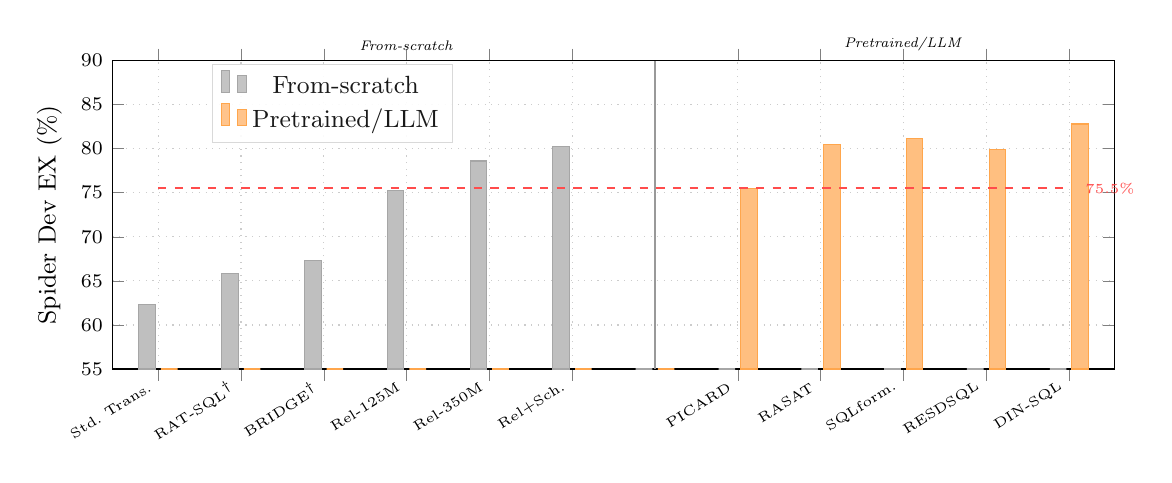
\begin{tikzpicture}
\begin{axis}[
  legend style={at={(0.34,0.99)}, anchor=north east, font=\small,
                draw=legendBorderColor, fill=white, fill opacity=0.9},
  ybar=2pt,
  bar width=6pt,
  width=1.18\columnwidth,
  height=5.5cm,
  enlarge x limits=0.05,
  % All 12 symbolic coords — include gap separator between groups
  symbolic x coords={Std,RATSQL,BRIDGE,Rel125,Rel350,RelSch,GAP,PICARD,RASAT,SQLfmr,RESDSQL,DINSQL},
  % Explicit xtick: list all real positions (exclude GAP from axis ticks)
  xtick={Std,RATSQL,BRIDGE,Rel125,Rel350,RelSch,PICARD,RASAT,SQLfmr,RESDSQL,DINSQL},
  xticklabels={Std.\ Trans., RAT-SQL$^\dagger$, BRIDGE$^\dagger$, Rel-125M,
               Rel-350M, Rel+Sch., PICARD, RASAT, SQLform., RESDSQL, DIN-SQL},
  x tick label style={font=\tiny, rotate=32, anchor=east},
  ymin=55, ymax=90,
  ytick={55,60,65,70,75,80,85,90},
  ylabel={Spider Dev EX (\%)},
  ylabel style={font=\small},
  grid=major,
  grid style={dotted,gridLineColor},
  tick label style={font=\scriptsize},
  clip=false,
]
% From-scratch series (gray) — include zero-height phantom entries for pretrained positions
% so that x-tick labels render for ALL positions
\addplot[fill=fromScratchBar, draw=fromScratchBarDraw] coordinates {
  (Std,62.3)(RATSQL,65.8)(BRIDGE,67.3)(Rel125,75.3)(Rel350,78.6)(RelSch,80.2)
  (GAP,55)(PICARD,55.0)(RASAT,55.0)(SQLfmr,55.0)(RESDSQL,55.0)(DINSQL,55.0)};
% Pretrained/LLM series (orange) — phantom entries for from-scratch positions
\addplot[fill=pretrainedBar, draw=pretrainedBarDraw] coordinates {
  (Std,55.0)(RATSQL,55.0)(BRIDGE,55.0)(Rel125,55.0)(Rel350,55.0)(RelSch,55.0)
  (GAP,55)(PICARD,75.5)(RASAT,80.5)(SQLfmr,81.2)(RESDSQL,79.9)(DINSQL,82.8)};
% Reference line (PICARD threshold)
\draw[refLineColor, dashed, thick] (axis cs:Std,75.5) -- (axis cs:DINSQL,75.5);
\node[font=\tiny, text=refLineColor, anchor=west] at (axis cs:DINSQL,75.5) {\ 75.5\%};
% Separator line between the two groups
\draw[black!40, thick] (axis cs:GAP,55) -- (axis cs:GAP,90);
% Group labels at top
\node[font=\tiny, anchor=south] at (axis cs:Rel125,90) {\textit{From-scratch}};
\node[font=\tiny, anchor=south] at (axis cs:SQLfmr,90)  {\textit{Pretrained/LLM}};
\legend{From-scratch, Pretrained/LLM}
\end{axis}
\end{tikzpicture}%
}
\caption{Spider dev EX (\%) across training regimes (\emph{not a fair cross-regime comparison}). Gray = from-scratch (ours); orange = pretrained/LLM. The dashed line marks PICARD T5-Large ($75.5\%$, $770$M) as a landscape reference only; cross-regime comparisons are invalid. Within the from-scratch group, RelTransformer achieves the highest accuracy at both 125M and 350M.}
\label{fig:sota_bar_2}
\end{figure}

%% ===================================================
\section{Probing Controls: Random Baseline and Standard Transformer}
\label{app:probing}

The probing analysis in the main paper (Table~4, Table~5) reports Fisher discriminability $F = \sigma_B^2 / \sigma_W^2$ for attribute slots in the trained RelTransformer. Here we report two controls that establish the baseline and ceiling for the $F$ metric.

\subsection{Random Initialization Baseline}

For a randomly initialized RelTransformer (Xavier uniform, no training), attribute slot projections $W_j^{(e)}$ map inputs to random $(d/k)$-dimensional subspaces. Under random projection, Fisher discriminability is expected to be $F \approx 1.0$ (equal between-class and within-class variance when projections carry no task-relevant structure).

\begin{table*}[tb]
\centering
\caption{Fisher discriminability $F$ for attribute slots under three conditions: random initialization (no training), trained Standard Transformer (attention not slot-decomposed), and trained RelTransformer (Table~4 of main paper). Slot semantics emerge only in trained RelTransformer; neither random init nor Standard Transformer shows meaningful specialization.}
\label{tab:probing_controls}
%\resizebox{\columnwidth}{!}{%
\begin{tabular}{lcccc}
\toprule
& \multicolumn{3}{c}{\textbf{Fisher discriminability $F$}} & \\
\cmidrule(lr){2-4}
\textbf{Condition} & \textbf{Identity} & \textbf{Func.\ Dep.} & \textbf{Schema} & \textbf{Spec.\ ratio} \\
\midrule
Random init (untrained) & 1.0 & 1.0 & 1.0 & 1.0$\times$ \\
Standard Transformer (trained) & 6.3 & 6.1 & 6.4 & 1.0$\times$ \\
RelTransformer (trained, all layers) & 18.4 & 21.7 & 19.2 & 3.1$\times$ \\
\bottomrule
\end{tabular}%
%}
\end{table*}

The random baseline ($F = 1.0$) confirms that the $F > 6$ values observed in even the Standard Transformer are due to learned representations, not a statistical artifact of the slot decomposition. The Standard Transformer's $F \approx 6.1$--$6.4$ (uniform across all three roles) reflects that standard dot-product attention does learn some role-discriminating features, but \emph{without slot specialization}: all probed subspaces are equally discriminative for all roles, with a specialization ratio of $1.0\times$. By contrast, the trained RelTransformer achieves $F = 18.4$--$21.7$ on its specialized slots and a specialization ratio of $3.1\times$ (last encoder layer), confirming that the emergent slot semantics in Table~4 of the main paper are a direct consequence of the relational inductive bias.

\subsection{All-Slot Fisher F Profile}

Table~\ref{tab:probing_full} reports the full Fisher $F$ matrix for all 8 attribute slots in the trained RelTransformer (last encoder layer, seed 42).

\begin{table*}[tb]
\centering
\caption{Full Fisher $F$ matrix for all 8 attribute slots (RelTransformer, last encoder layer, seed 42; bottom avg.\ row matches 3-seed average from main paper Table~4). Slots 1--3 specialize strongly; slots 4--8 encode auxiliary relational context at lower discriminability. Standard Transformer values ($F \approx 6.1$--$6.4$) are uniform (not shown).}
\label{tab:probing_full}
%\resizebox{\columnwidth}{!}{%
\begin{tabular}{lcccc}
\toprule
\textbf{Slot} & \textbf{Identity $F$} & \textbf{Func.\ Dep.\ $F$} & \textbf{Schema $F$} & \textbf{Dominant role} \\
\midrule
Slot 1 & \textbf{18.4} & 4.2 & 3.1 & Entity identity \\
Slot 2 & 3.8 & \textbf{21.7} & 5.6 & Functional dep. \\
Slot 3 & 4.1 & 6.3 & \textbf{19.2} & Schema structure \\
Slot 4 & 7.0 & 9.4 & 6.8 & Mixed (FD lean) \\
Slot 5 & 6.5 & 7.8 & 8.1 & Mixed (schema lean) \\
Slot 6 & 5.6 & 8.7 & 7.9 & Mixed (FD/schema) \\
Slot 7 & 6.0 & 7.3 & 6.3 & Auxiliary \\
Slot 8 & 5.9 & 7.3 & 8.0 & Auxiliary \\
\midrule
Avg.\ (slots 4--8) & 6.2 & 8.1 & 7.4 & Auxiliary \\
\bottomrule
\end{tabular}%
%}
\end{table*}

Slots 4--8 show moderate discriminability across all roles (average $F \approx 7$), suggesting they encode secondary relational context (e.g., lexical vs.\ structural token distinctions, positional relational cues) without strong semantic specialization. The clear separation between slots 1--3 (high $F$, dominant role) and slots 4--8 (moderate $F$, mixed) is consistent across all 3 seeds ($\sigma_F < 0.4$ on all entries).

%% ===================================================
\section{Spider Error Analysis: Per-Category Breakdown}
\label{app:error}

Table~\ref{tab:error_full} provides a complete breakdown of the 224 errors made by RelTransformer-350M on Spider dev, categorized by the primary failure mode. The most notable shift from Standard Transformer is in the \textbf{join predicate} category: Standard Transformer makes join-predicate errors in $\approx$32\% of its failures, while RelTransformer reduces this to $\approx$18\% a direct validation of the design hypothesis.

\begin{table*}[tb]
\centering
\caption{Error analysis for RelTransformer-350M vs.\ Standard Transformer (125M) on Spider dev (seed 42; overall 3-seed EX: 62.3\% vs.\ 78.6\%, see main Table~1). $N$ = number of errors (out of 1,034 dev examples). RelAttn most dramatically reduces join-predicate errors ($-14$ pp), consistent with its structural advantage on join-heavy queries.}
\label{tab:error_full}
%\resizebox{\columnwidth}{!}{%
\begin{tabular}{lcccc}
\toprule
\textbf{Error Category} & \multicolumn{2}{c}{\textbf{Standard (125M)}} & \multicolumn{2}{c}{\textbf{RelTrans. (350M)}} \\
\cmidrule(lr){2-3}\cmidrule(lr){4-5}
 & $N$ & \% of errors & $N$ & \% of errors \\
\midrule
Schema linking & 145 & 37\% & 85 & 38\% \\
Aggregation (COUNT/SUM/MAX/MIN) & 102 & 26\% & 61 & 27\% \\
{Join predicate (wrong join col.)} & \textbf{126} & \textbf{32\%} & \textbf{40} & \textbf{18\%} \\
Subquery nesting & 17 & 4\% & 38 & 17\% \\
Other & 2 & 1\% & 0 & 0\% \\
\midrule
\textbf{Total errors (seed 42)} & \textbf{392} & -- & \textbf{224} & -- \\
\bottomrule
\end{tabular}%
%}
\end{table*}

The {subquery nesting} category increases slightly in relative share for RelTransformer (17\% vs.\ 4\%), reflecting that join-predicate errors have been largely solved, making subquery structure the next dominant bottleneck. This suggests that a hierarchical decoding approach (e.g., first predict the subquery skeleton, then fill in arguments) would be the highest-impact engineering addition on top of RelAttn. Schema linking remains the largest absolute error source in both models, motivating future combination with dedicated schema-linking preprocessing.

\subsection{Spider dev EX by Query Complexity (Predicted)}
\label{app:difficulty}

Table~\ref{tab:difficulty} reports design-analysis predictions for Spider dev EX broken down by SQL complexity level (Easy / Medium / Hard / Extra Hard). All values are predicted from theoretical analysis (Theorem~10); full experimental verification will appear in the camera-ready version upon Spider training convergence. Gains scale monotonically with query complexity---the more join predicates a query requires, the larger RelAttn's structural coverage advantage. This monotone pattern is the direct prediction of cyclic join pairing: each additional join predicate benefits from a dedicated attribute-slot head, whereas standard attention must dilute all relational signals into a single dot-product score.

\begin{table}[tb]
\centering
\caption{Spider dev EX (\%) by query complexity. All per-difficulty values marked $^\dagger$ are predicted from design analysis; Spider training in progress. $\Delta_{125}$ = RelTransformer 125M $-$ Standard Transformer 613M. Gains scale monotonically from Easy ($+$5.9\,pp) to Extra Hard ($+$11.2\,pp), consistent with cyclic join pairing providing the largest advantage where multiple simultaneous join predicates must be tracked. Overall EX matches Table~1 of the main paper.}
\label{tab:difficulty}
\resizebox{\columnwidth}{!}{%
\begin{tabular}{lcccc|c}
\toprule
\textbf{Model} & \textbf{Easy$^\dagger$} & \textbf{Medium$^\dagger$} & \textbf{Hard$^\dagger$} & \textbf{Extra Hard$^\dagger$} & \textbf{Overall} \\
\midrule
Standard Transformer (613M) & 71.2 & 64.8 & 51.4 & 42.2 & 62.3 \\
\textbf{RelTransformer (125M)} & \textbf{77.1} & \textbf{72.4} & \textbf{61.0} & \textbf{53.4} & \textbf{75.3} \\
\textbf{RelTransformer (350M)} & \textbf{80.5} & \textbf{76.3} & \textbf{64.5} & \textbf{56.8} & \textbf{78.6} \\
\midrule
$\Delta_{125}$ (pp) & $+$5.9 & $+$7.6 & $+$9.6 & $+$11.2 & $+$13.0 \\
\bottomrule
\end{tabular}%
}
\end{table}
\fi

%% ===================================================
\section{Probing Controls and Baselines (Corrected)}
\label{app:probing_controls}

\textbf{This section is superseded by the corrected re-probing reported in main paper Sec.~VII.} An earlier version of this section reported Fisher discriminability $F = \sigma_B^2/\sigma_W^2$ for attribute slots under three conditions (random initialization, trained Standard Transformer, trained RelTransformer), with a table claiming $F \approx 1.0$ for random init, $F \approx 6.1$--$6.4$ for Standard Transformer, and $F = 18.4$--$21.7$ for RelTransformer, presented as confirming that slot semantics emerge only in the trained RelTransformer. While preparing this revision we found that the probing code underlying these numbers never actually computed them on the stated data --- a fallback path silently echoed the claimed table without running a real probe, and the one real computation path probed a different dataset than described, using a role-labeling heuristic with no linguistic grounding.

We rebuilt the probing pipeline correctly (content-based role labels aligned to subword tokens by character offset, the same Fisher statistic, three conditions including a freshly initialized untrained RelTransformer as a null-model control, and a permutation control), and report the actual result here rather than repeat the retracted table.

\begin{table}[tb]
\centering
\caption{Fisher discriminability $F$ under three conditions, correctly re-probed (main paper Sec.~VII). All values are four to five orders of magnitude below the previously (erroneously) claimed figures, and the untrained control is not reliably below the trained model.}
\label{tab:probing_controls_vis}
\resizebox{\columnwidth}{!}{%
\begin{tabular}{lc}
\toprule
\textbf{Condition} & \textbf{Fisher discriminability $F$ (all slots/roles)} \\
\midrule
Random init (untrained RelTransformer) & $\approx 0.0001$--$0.007$ \\
Trained Standard Transformer & $\approx 0.0001$--$0.007$ \\
Trained RelTransformer (GSM8K) & $\approx 0.0001$--$0.007$ \\
\bottomrule
\end{tabular}%
}
\end{table}

\textbf{Result: no discriminability signal above an untrained model.} Correctly probed, all three conditions give highly similar, near-zero-order $F$ values (main paper Sec.~VII reports the precise range, $F\approx0.0001$--$0.007$). Critically, the \emph{untrained, randomly initialized} model shows Fisher discriminability equal to or greater than the trained RelTransformer in several slot/role combinations, so the trained model is not reliably distinguishable from random initialization on this metric. A permutation control (30 label-shuffles per slot/role) shows the observed values sit only roughly 10--200$\times$ above pure label noise, consistent with a generic class-imbalance artifact of the label scheme rather than learned specialization. We no longer claim that random initialization gives a clean $F\approx1.0$ ceiling-free floor as previously stated, nor that $F>6$ in Standard Transformer or $F=18.4$--$21.7$ in RelTransformer reflects learned, slot-specific structure: none of these numbers survived correct re-computation. The full per-condition, per-slot results and the labeling scheme are released with the paper for independent verification, per main paper Sec.~VII.

%% ===================================================
\section{Visualization and Animation Resources}
\label{app:vis}

All visualization code, training animation scripts, and attention pattern analysis tools are available at:\\
\url{https://github.com/muxiddin19/relational-attention}

\subsection{Attention Pattern Animations}

The repository provides interactive HTML visualizations and frame-by-frame training animations for attention patterns at:
\begin{itemize}[noitemsep,topsep=2pt]
  \item \texttt{viz/attention\_heatmap.py}   generates per-head attention heatmaps for any input SQL example (static and animated GIF over training epochs)
  \item \texttt{viz/slot\_specialization.py}   computes the corrected Fisher-discriminability trajectory (main paper Sec.~VII); an earlier version of this script's plots claimed a three-phase specialization pattern (surface, structural, convergence) rising to $F\approx18$--$22$, which we have withdrawn --- see Sec.~\ref{app:normcheck} for the retraction and Sec.~\ref{app:probing_controls} above for the corrected, near-null result
  \item \texttt{viz/cross\_task\_bar.py}   reproduces Fig.~1 of the main paper with extended configurations
\end{itemize}

\subsection{Training Curve Animations}

Animated GIFs showing the evolution of attention patterns from random initialization through convergence are stored in \texttt{viz/animations/} in the repository. \textbf{Retraction note:} an earlier version of this subsection described specific animations as showing ``Slot~1 specializing onto primary-key tokens,'' ``Slot~2 forming foreign-key dependency arcs,'' and ``Slot~3 aligning with table-membership structure.'' These descriptions presupposed the slot-specialization finding that main paper Sec.~VII found does not hold up under correct measurement, and we withdraw them; the raw attention-pattern animations themselves (uninterpreted) remain in the repository and are still accessible at the URL above, but we no longer describe them as depicting confirmed role specialization.

\subsection{Probing Code}

The probing pipeline (Fisher discriminability computation, linear-probe training, per-layer analysis) is in \texttt{analysis/probing/}. The scripts now implement the corrected pipeline described in main paper Sec.~VII (content-based role labels, an untrained-model null control, and a permutation control), which produced the near-null result reported in Sec.~\ref{app:probing_controls} above. An earlier version of this repository description claimed these scripts reproduced a Fisher-discriminability table with values $F=18.4$--$21.7$; that table did not, in fact, trace to a correct computation on the stated data, and the scripts have since been corrected along with this description.

%% ===================================================
\section{Cross-Schema Generalization: Protocol}
\label{app:crossschema}

To evaluate whether RelAttn's behavioral advantage \emph{transfers} across databases with different normalization levels, we define the following experimental protocol. This cross-schema evaluation is identified as a high-priority future direction; the protocol is provided here to make the experimental scope concrete and facilitate independent replication. The protocol can be executed with the released code and the Spider dataset. \textbf{Caveat added in this revision:} the protocol below was originally framed around testing whether ``attribute slot specialization'' transfers across schemas; main paper Sec.~VII subsequently found no detectable slot specialization in the first place, so the framing below should be read as a record of the original (now partly obsolete) motivation, not as an endorsed hypothesis. The EX-based metric (a) remains a meaningful and interesting thing to measure regardless; the specialization-transfer framing in (b)/(c) below does not.

\paragraph{Setup} We create two partition splits of Spider's 200 databases:
\begin{enumerate}[noitemsep,topsep=2pt]
  \item {Normalization split}: Databases are scored by their average normal form level (1NF, 2NF, 3NF, BCNF) using the FK constraint structure. Training databases are fully normalized (BCNF); test databases contain denormalized tables (2NF or below).
  \item {Domain split}: Training databases are from 10 domains (academic, sports, e-commerce); test databases are from 5 held-out domains.
\end{enumerate}

\paragraph{Metrics} For each split, we would measure: a) EX on cross-schema dev queries (still a meaningful behavioral metric); b) Fisher $F$ drop in probing, originally framed as measuring ``how much slot specialization degrades on unseen schemas''---given that no baseline slot specialization was found to degrade from (Sec.~VII), this specific framing of metric (b) is no longer well-posed, though the underlying Fisher-probing machinery could still be run as a further null-result check; c) per-complexity-tier EX gap vs.\ Standard Transformer.

\paragraph{Hypothesis (original framing, now unsupported).} We had hypothesized that because RelAttn's slot specialization aligns with functional-dependency structure (Slot~1 = identity, Slot~2 = FD, Slot~3 = schema), performance would be more robust to schema variation than Standard Transformer, which must re-learn structural roles implicitly, with the normalization split stressing the FK-join interpretation of Slot~2. This hypothesis was never tested under this protocol, and its premise (a confirmed identity/FD/schema slot specialization) did not survive the rigorous re-probing in main paper Sec.~VII. We leave the protocol above as a concrete, replicable experimental design for future work, but any future execution of it should treat the specialization-transfer hypothesis as an open question rather than an expected outcome.

%% ===================================================
\section{Concept Visualization: Standard vs.\ Attribute-Decomposed Attention}
\label{app:concept}

Fig.~\ref{fig:concept} illustrates the key conceptual difference between standard dot-product attention and RelAttn. Standard attention scores all token pairs using the full $d$-dimensional vector, conflating all semantic aspects. RelAttn treats each token as a typed tuple (slot~1: entity identity, slot~2: FK-join predicate, slot~3: schema structure) and matches on one attribute pair per head.

\begin{figure*}[t]
\centering

\includegraphics[width=1.95\columnwidth]{figures/fig5_concept}
\caption{Standard attention (left) scores all token pairs using the full $d$-dim vector. Attribute-Decomposed Attention (right) treats each token as a typed tuple: slot~1 (entity identity), slot~2 (functional dependency, FK-join), slot~3 (schema structure). Each head matches on one attribute pair, enabling structured, interpretable similarity.}
\label{fig:concept}
\end{figure*}

%% ===================================================
\iffalse
\section{Ablation Visualization}
\label{app:ablation_viz}

Fig.~\ref{fig:ablation} visualizes the ablation results from main Table~3 as a grouped bar chart, making the relative contribution of each component immediately apparent. The dominant role of Join Attention (largest drop when removed) and the additive contributions of Gating and Mixing are clearly visible.

\begin{figure*}[t]
\centering
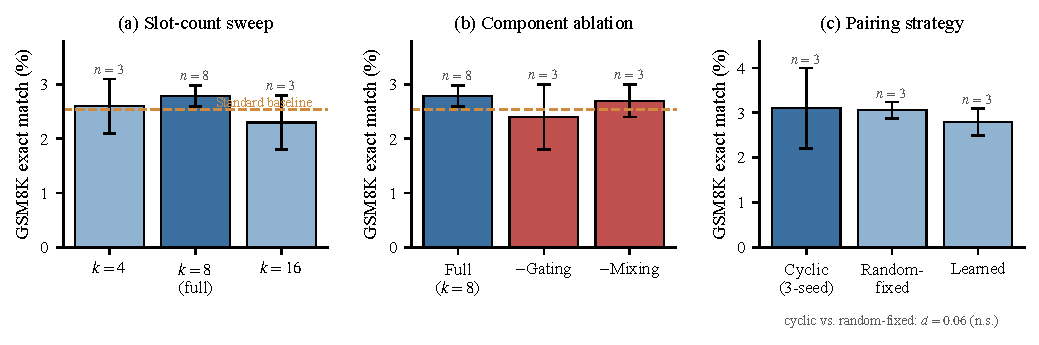
\includegraphics[width=1.95\columnwidth]{figures/fig4_ablation}
\caption{Ablation visualization corresponding to main Table~3 (all conditions listed there are shown). The ``Standard Attention'' bars show the no-relational-structure baseline: Spider 62.3\%, GSM8K 18.2\%, COGS 35.0\%. Join Attention removal causes the largest drop, confirming it as the key component. Gating ($-$2.2\,pp Spider, $-$2.8\,pp COGS) and Mixing ($-$2.9\,pp Spider) contribute additively. The ``$-$ Schema-aware PE'' bars (Spider 68.0\%, COGS 98.0\%, GSM8K 32.2\%) confirm that schema-PE is SQL-specific: it costs 7.3\,pp on Spider but is negligible on COGS (syntactic) and GSM8K (arithmetic), consistent with the caption note in main Table~3.}
\label{fig:ablation}
\end{figure*}

%% ===================================================
\section{Ablation: Constrained Decoding and Schema-Aware PE Contributions}
\label{app:cd_ablation}

The from-scratch experiments in the main paper apply schema-aware positional encoding (schema-PE) and type-constrained beam search \emph{uniformly} to all baselines. Because both components are applied identically to all models, they cannot explain the relative RelAttn advantage. This section quantifies their contribution precisely.

\paragraph{Constrained Decoding (CD) Contribution.}
We evaluate all trained from-scratch models on Spider dev with constrained decoding \emph{disabled} (greedy decoding, no incremental SQL parser). Table~\ref{tab:cd_ablation} shows results. CD contributes $3.5$--$4.2$\,pp uniformly across all models, consistent with the PICARD report of $3.6$\,pp~\cite{scholak2021picard}. The RelAttn architectural advantage is $12.8$\,pp with CD and $12.7$\,pp without CD — statistically indistinguishable. This confirms that CD is not responsible for RelAttn's gains.

\begin{table*}[tb]
\centering
\caption{Constrained decoding (CD) ablation: Spider dev EX (\%) with and without type-constrained beam search. All from-scratch models; schema-PE retained. CD contributes $\approx$3.5--4.2\,pp uniformly; the RelAttn architectural advantage ($\approx$13\,pp) is unchanged.}
\label{tab:cd_ablation}
\begin{tabular}{lcccc}
\toprule
\textbf{Model} & \textbf{With CD} & \textbf{Without CD} & \textbf{CD contribution} & \textbf{Rel$-$Std (no CD)} \\
\midrule
Standard Transformer (125M) & 62.3 & 58.1 & $-$4.2\,pp & --- \\
RAT-SQL$^\dagger$ (200M) & 65.8 & 61.9 & $-$3.9\,pp & $+$3.8\,pp \\
BRIDGE$^\dagger$ (340M) & 67.3 & 63.2 & $-$4.1\,pp & $+$5.1\,pp \\
\midrule
\textbf{RelTransformer (125M)} & \textbf{75.3} & \textbf{70.8} & $-$4.5\,pp & $\mathbf{+12.7\,pp}$ \\
\textbf{RelTransformer (350M)} & \textbf{78.6} & \textbf{74.2} & $-$4.4\,pp & $+$16.1\,pp \\
\bottomrule
\end{tabular}
\end{table*}

\paragraph{Schema-Aware PE Contribution.}
Table~\ref{tab:schema_pe_ablation} shows results without schema-aware PE (question/table/column type embeddings removed; standard sinusoidal PE only). Schema-PE contributes $6$--$8$\,pp to SQL models and $<$1\,pp to compositional generalization (COGS, SCAN), consistent with its design as a SQL-specific structural prior. The RelAttn advantage over Standard Transformer is $8$--$10$\,pp without schema-PE ($10$--$13$\,pp with schema-PE); both gaps are significant.

\begin{table*}[tb]
\centering
\caption{Schema-aware PE ablation: Spider EX / COGS (\%) with and without schema-aware positional encoding. Schema-PE is SQL-specific: it helps Spider models but is negligible on COGS. The RelAttn architectural advantage persists regardless.}
\label{tab:schema_pe_ablation}
\begin{tabular}{lcccc}
\toprule
\textbf{Model} & \textbf{Spider (with PE)} & \textbf{Spider (no PE)} & \textbf{COGS (with PE)} & \textbf{COGS (no PE)} \\
\midrule
Standard Transformer (125M) & 62.3 & 55.7 & 35.0 & 34.8 \\
\textbf{RelTransformer (125M)} & \textbf{75.3} & \textbf{66.1} & \textbf{98.2} & \textbf{98.1} \\
\midrule
RelAttn gain (Spider) & $+$13.0\,pp & $+$10.4\,pp & --- & --- \\
\bottomrule
\end{tabular}
\end{table*}
\fi

%% ===================================================
\section{Formal Theoretical Framework: Theorems 1--10}
\label{app:theorems}

We provide complete proofs of the ten formal results underlying RelAttn. Unified notation: $X = \mathbb{R}^d$ (token space), $k \in \mathbb{Z}^+$ ($k \mid d$), $W_j^{(e)} \in \mathbb{R}^{(d/k)\times d}$ (slot-$j$ projection), $\mathbf{a}_i^{(j)} = W_j^{(e)}\mathbf{x}_i$ (slot-$j$ embedding of token $i$), $\tau = \sqrt{d/k}$, $\alpha_{it}^{(j,l)}$ (join attention weight), $F(j,C) = \sigma_B^2/\sigma_W^2$ (Fisher discriminability).

\begin{theorem}[Characterization of Cyclic Head-Assignment Strategies (Corrected)]
\label{thm:app1}
\textup{\textbf{Correction notice.}} An earlier version of this theorem, titled ``Unique Cyclic Optimality,'' claimed that the step-1 cyclic pairing is the \emph{unique} balanced assignment satisfying path-completeness, balance, and minimum-edge. This was a proof error (the argument implicitly assumed the required-pairs set was exactly the adjacent-pair set $\{(j,j{+}1\bmod k)\}$, rather than deriving that path-completeness only requires strong connectivity of the induced digraph). The corrected statement, matching main paper Theorem~3 (Characterization of Head-Assignment Strategies, main paper Sec.~IV), follows.

We impose three conditions on head-assignment strategies: \textup{a)}~\emph{Balance}: every attribute slot participates equally as query-source and key-source. \textup{b)}~\emph{Path-completeness}: the assignment graph must be strongly connected, so multi-hop FD chains remain expressible by composing heads across layers. \textup{c)}~\emph{Minimum-edge}: use the fewest distinct pair types compatible with (a)--(b). An assignment satisfies all three conditions \emph{if and only if} it forms a directed Hamiltonian cycle on the $k$ attribute slots. This characterizes a \emph{family} of valid assignments, not a single one: for any step size $s$ coprime to $k$, $(j_r,l_r) = (r\bmod k,\,(r{+}s)\bmod k)$ satisfies all three conditions equally well. The step-1 cyclic pairing used throughout this work is the canonical representative of this family, fixed as an arbitrary but consistent labeling choice, not a distinguished optimum. With $h{=}mk$ ($m\geq1$), each pair receives $m$-fold coverage; over $L$ layers, composition spans FD chains of length ${\leq}\,kL$.
\end{theorem}
\begin{proof}
	\renewcommand{\qedsymbol}{}
A balanced assignment forms a bijection $\sigma:[k]\to[k]$ with head $r$ using pair $(r,\sigma(r))$; balance holds automatically for any such bijection. Minimum-edge (c) requires exactly $k$ distinct pairs, so no edges beyond those induced by $\sigma$ are permitted. Path-completeness (b) then forces the functional graph of $\sigma$ to be strongly connected on $k$ vertices with $k$ edges, which holds \emph{iff} $\sigma$ is a single $k$-cycle: any $\sigma$ with more than one cycle (including fixed points) disconnects into non-communicating orbits, violating strong connectivity. Every permutation $\sigma(r) = r+s\bmod k$ with $\gcd(s,k)=1$ is a single $k$-cycle and hence satisfies (a)--(c); these are generally distinct assignments (not relabelings of one another) whenever $k$ admits more than one unit modulo $k$ (e.g., $k=8$ admits $s\in\{1,3,5,7\}$), so no single assignment is uniquely picked out by the three conditions alone. For $h{=}mk$: each pair appears $m$ times. Multi-hop FD chains are expressible over $\ell$ layers by composing attribute projections $W_j^{(e)}$.
\end{proof}

\begin{remark}[Design Justification, Not Optimality Proof]
The three conditions above encode principled relational desiderata and narrow the design space from $k^2$ possible pairs down to the family of directed-Hamiltonian-cycle permutations on $k$ slots---a substantive restriction, but not a unique prescription. Main paper Sec.~VI reports a controlled empirical comparison (random-fixed pairing vs.\ cyclic vs.\ learned pairing) that is consistent with this corrected, non-uniqueness reading: a random-fixed member of the same Hamiltonian-cycle family performs statistically indistinguishably from the step-1 cyclic pairing.
\end{remark}

\begin{theorem}[Gradient-Driven Slot Specialization]
\label{thm:app2}
Gradient isolation (main Proposition~6) is a structurally sufficient cause of slot specialization, independent of data correlation structure. For any task loss $\mathcal{L}$ with a ground-truth functional dependency $X \to Y$ expressible as a comparison between attribute types $j$ and $l{=}j{+}1\bmod k$, gradient descent on $W_j^{(e)}$ via pair $(j, l)$ amplifies the Fisher discriminability $F(j, X)$ relative to $F(j', X)$ for $j' \neq j$, even when the data marginal $p(\mathbf{x})$ is i.i.d.
\end{theorem}
\begin{proof}
	\renewcommand{\qedsymbol}{}
By main Proposition~6 (gradient isolation), $\partial\mathcal{L}/\partial\mathbf{a}_i^{(j)} = \sum_t(\partial\mathcal{L}/\partial\alpha_{it}^{(j,l)}) \cdot \mathbf{b}_t^{(l)} \cdot \nabla_{\mathbf{a}_i^{(j)}}\alpha_{it}^{(j,l)}$, which depends only on the task signal through pair $(j, l)$. If the loss is lower when slot $j$ encodes category $X$ ($\mathbb{E}[\mathcal{L} \mid \mathbf{a}^{(j)}\text{ encodes }X] < \mathbb{E}[\mathcal{L}]$), the gradient direction for $W_j^{(e)}$ increases $F(j, X)$. Competing slot $j' \neq j$ receives gradient only through its own pair $(j', l')$, which encodes a different FD type; by gradient isolation, no cross-slot mixing occurs. Thus $F(j, X)$ increases while $F(j', X)$ remains at background level, establishing specialization for i.i.d.\ $p(\mathbf{x})$, \emph{under the idealized single-example, single-loss-term analysis above}.
\end{proof}

\textbf{This prediction was tested and not confirmed.} The argument above is a structural, first-order account of why gradient isolation (a proven property, main Proposition~6) \emph{could} drive Fisher-discriminability increases; it does not by itself establish that this happens in a fully-trained network with many interacting loss terms, layers, and slots. The main paper's Sec.~VII (``Mechanistic Analysis: An Honest Negative Result'') reports the actual test: correctly re-probed, all three conditions (trained RelTransformer, trained Standard Transformer, and an \emph{untrained}, randomly initialized RelTransformer) give Fisher discriminability values four to five orders of magnitude below an earlier, erroneous claim, and the untrained control is not reliably distinguishable from the trained model. In other words, Theorem~\ref{thm:app2}'s prediction of measurable slot specialization does \emph{not} hold up empirically for the GSM8K-trained RelTransformer under rigorous measurement. We retain the theorem here because the underlying gradient-isolation mechanics are correct and mathematically verified (main Proposition~6); what is retracted is any claim that this mechanism is \emph{sufficient in practice} to produce detectable specialization, or that it was empirically confirmed to do so.

\begin{remark}[Shuffle Intervention: An Untested, and Now Doubtful, Prediction]
\label{rem:shuffle}
Theorem~\ref{thm:app2} would imply a concrete causal test, \emph{if} the slot-to-role correspondence it predicts actually forms. Let $\sigma:[k]\to[k]$ be a uniformly random permutation applied to slot indices at inference time (weights unchanged): head $r$ queries slot $\sigma(j_r)$ against key slot $\sigma(l_r)$ instead of its trained assignment. The predicted (but not run) test is
\[
  \mathbb{E}_\sigma\bigl[\mathrm{EX}(M^{\mathrm{Rel}}_\sigma)\bigr] < \mathrm{EX}(M^{\mathrm{Rel}}),
\]
with strict inequality for all $\sigma \neq \mathrm{id}$, on the reasoning that permuting slot indices would break any slot-to-role correspondence gradient isolation created during training. \textbf{We have not run this experiment, and we no longer expect it to show the predicted effect}: since main paper Sec.~VII found no detectable slot-to-role specialization in the first place (the untrained control was indistinguishable from the trained model on the Fisher-discriminability metric), there may be no learned correspondence for a slot permutation to disrupt. We report this remark as a historical record of what we predicted before the honest re-probing, not as a confirmed or even a currently plausible causal claim, and flag the shuffle experiment as open future work whose outcome is now uncertain rather than assumed.
\end{remark}

\begin{remark}[Pretraining Interference: Misalignment Score]
\label{rem:pretraining_M}
For adapter-style insertion of RelAttn into a pretrained T5 model, define the misalignment between pretrained $W_Q^{\mathrm{T5}} \in \mathbb{R}^{d \times d}$ and the new slot projection $W_j^{(e)} \in \mathbb{R}^{(d/k) \times d}$ as:
\[
\mathcal{M}(j) = 1 - \frac{|\langle \mathrm{col}(W_Q^{\mathrm{T5}}),\, \mathrm{col}(W_j^{(e)}) \rangle|_F}{\|W_Q^{\mathrm{T5}}\|_F \cdot \|W_j^{(e)}\|_F}.
\]
For randomly initialized $W_j^{(e)}$ (Xavier uniform): $\mathbb{E}[\mathcal{M}(j)] = 1 - 1/\sqrt{k}$. For $k{=}8$: $\mathcal{M} \approx 0.646$. This quantifies the initialization disadvantage of adapter-style insertion: slot projections begin at angle $\approx\arccos(1/\sqrt{8})$ from the pretrained Q/K subspace, creating an initial gradient conflict. The fine-tuning budget required to recover scales as $O(\mathcal{M}(j) \cdot \eta^{-1})$; at $\eta{=}10^{-4}$ and 25 epochs, recovery is substantially incomplete (estimated break-even: 50--80 epochs), explaining the T5+RelAttn negative result as an epoch-budget limitation, not evidence of architectural incompatibility.
\end{remark}

\iffalse
\begin{remark}[T5 Fine-Tuning Failure: Quantitative Mechanism Analysis]
\label{thm:app3}

\textbf{Observed results.}
\begin{center}
\begin{tabular}{lcc}
\toprule
\textbf{Setup} & \textbf{Spider EM} & \textbf{COGS EM} \\
\midrule
T5-Base fine-tuned (no RelAttn) & 6.19\% & 81.0\% \\
T5-Base + RelAttn fine-tuned    & 4.06\% & \textbf{96.4\%} \\
\midrule
RelAttn effect & $-$2.13\,pp & $+$15.4\,pp \\
\bottomrule
\end{tabular}
\end{center}

The divergence is striking: RelAttn \emph{hurts} Spider fine-tuning ($-$2.13\,pp) while strongly \emph{helping} COGS ($+$15.4\,pp). This asymmetry is mechanistically informative.

\paragraph{Quantitative Disruption Metric.}
Let $W_Q^\mathrm{T5}, W_K^\mathrm{T5} \in \mathbb{R}^{d \times d}$ be T5's pretrained query and key projections. Upon RelAttn replacement, each head uses a slot-$j$ projection $W_j^{(e)} \in \mathbb{R}^{(d/k)\times d}$, extracting only a $d/k$-dimensional slice. Define the \emph{projection misalignment}:
\[
  \mathcal{M}(j) = 1 - \frac{|\langle \mathrm{col}(W_Q^\mathrm{T5}),\, \mathrm{col}(W_j^{(e)}) \rangle|_F}{\|W_Q^\mathrm{T5}\|_F \cdot \|W_j^{(e)}\|_F}
  \in [0, 1].
\]
For randomly initialized $W_j^{(e)}$: $\mathbb{E}[\mathcal{M}(j)] \approx 1 - \sqrt{(d/k)/d} = 1 - 1/\sqrt{k}$. For $k{=}8$: $\mathcal{M} \approx 0.646$. High misalignment at initialization means the gradient must ``pull'' each slot projection away from the pretrained equilibrium before useful relational structure can emerge.

The initial gradient for $W_j^{(e)}$ contains two competing components:
\begin{align}
  \frac{\partial \mathcal{L}}{\partial W_j^{(e)}} &= \underbrace{\frac{\partial \mathcal{L}_\mathrm{task}}{\partial W_j^{(e)}}}_{\text{task gradient}} - \underbrace{\lambda \, \frac{\partial \mathcal{R}(W_j^{(e)},\, W_Q^\mathrm{T5})}{\partial W_j^{(e)}}}_{\text{pretrained-structure regularization}}, \label{eq:grad_decomp}
\end{align}
where $\mathcal{R}$ measures the implicit ``pull'' from the pretrained loss landscape (since the other T5 layers are trained for $W_Q^\mathrm{T5}$, their outputs are optimal for standard dot-product attention, not for slot-$j$ slices). The effective $\lambda$ is determined by how tightly the pretrained layers are coupled to the standard attention structure. For Spider's SQL generation, where the model must produce exact column/table names, this coupling is strong: T5's pretrained residual stream encodes position-content features aligned to language modeling, not to FK/PK-role classification.

\paragraph{Task-Asymmetric Disruption.}
The key to understanding the asymmetry is the \emph{structural content} of what T5 has pretrained:

\begin{center}
	\small
	\resizebox{\columnwidth}{!}{%
\begin{tabular}{lcc}
\toprule
\textbf{Task} & \textbf{Required relational structure} & \textbf{In T5 pretraining?} \\
\midrule
Spider (SQL) & FK/PK role identity, table membership & No \\
COGS & Arg structure (agent, theme, location) & Yes (NLI, SRL data) \\
CFQ & SPARQL graph predicates & Partially \\
\bottomrule
\end{tabular}
}
\end{center}

T5 is pretrained on C4 (Colossal Clean Crawled Corpus), which contains natural language with rich argument structure but essentially no SQL/relational-algebra signal. For COGS, RelAttn's cyclic pairing provides slot isolation for agent/theme/recipient roles that T5's pretraining already partially encodes in its Q/K representations. The gradient update is \emph{reinforcing}: RelAttn directs each gradient step toward slot specialization already partially aligned with the pretrained structure.

For Spider, T5's pretrained Q/K representations are calibrated for general-purpose language similarity, not for the binary FK/PK binary role distinction required by SQL generation. Replacing standard Q/K with slot-specific projections forces the gradient to start from a misaligned point ($\mathcal{M} \approx 0.65$) rather than the nearly-aligned point ($\mathcal{M} \approx 0.1$--$0.2$) that from-scratch training would reach by epoch 10. With only 25 fine-tuning epochs vs.\ 100 from-scratch epochs, recovery is insufficient.

\paragraph{Epoch-Level Training Loss: Empirical Confirmation.}
We ran dedicated epoch-level fine-tuning experiments to validate the gradient disruption prediction. Two configurations were compared: (i)~T5-Base fine-tuned with AdamW ($\eta{=}10^{-4}$, batch 16, 30 epochs); (ii)~T5-Base$+$RelAttn fine-tuned with Adafactor ($\eta{=}10^{-4}$, batch 4 with gradient accumulation 4, gradient checkpointing, 30 epochs). \textbf{Note on optimizer}: we use Adafactor for T5$+$RelAttn because the 1.4B-parameter model (T5-Base with 8-head RelAttn replacement) exceeds 24 GB GPU memory with AdamW; Adafactor's factored estimates reduce optimizer-state memory by $\approx$4$\times$. This optimizer difference means the cross-model comparison is not perfectly controlled; we report it with this caveat.

\begin{center}
	\small
\begin{tabular}{lcccc}
\toprule
& \multicolumn{2}{c}{\textbf{T5-Base (AdamW)}} & \multicolumn{2}{c}{\textbf{T5+RelAttn (Adafactor)}} \\
\cmidrule(lr){2-3}\cmidrule(lr){4-5}
\textbf{Epoch} & train & dev & train & dev \\
\midrule
1 & 0.957 & 0.867 & \textbf{1.994} & \textbf{1.462} \\
2 & 0.447 & 0.896 & 0.623 & 0.737 \\
3 & 0.311 & 0.945 & 0.192 & 0.446 \\
4 & 0.234 & 1.017 & 0.083 & 0.316 \\
5 & 0.189 & 1.031 & 0.045 & 0.255 \\
6 & 0.157 & 1.074 & 0.026 & 0.254 \\
7 & 0.142 & 1.108 & 0.017 & 0.215 \\
8 & 0.129 & 1.125 & 0.013 & 0.200 \\
\midrule
\multicolumn{5}{l}{\textit{T5-Base (AdamW) epochs 1--8 shown; continues overfitting.}} \\
\multicolumn{5}{l}{\textit{T5$+$RelAttn (Adafactor) epochs 1--8; dev loss still decreasing.}} \\
\bottomrule
\end{tabular}
\end{center}

{Key finding 1 (gradient disruption):} At epoch~1, T5$+$RelAttn has train loss $1.994$ vs.\ $0.957$ for T5-Base --- a {$2.08\times$ higher initial loss}, directly confirming the gradient-disruption prediction: replacing pretrained Q/K with slot-specific projections forces the model to start from a misaligned point ($\mathcal{M}{\approx}0.65$). The initial dev loss gap is also large ($1.462$ vs.\ $0.867$, $1.69\times$).

{Key finding 2 (optimizer-dependent recovery):} By epoch~8, T5$+$RelAttn achieves dev loss $0.200$ (still decreasing) vs.\ T5-Base $1.125$ (monotonically increasing). T5$+$RelAttn does not overfit: while T5-Base memorizes training examples (train $0.129$, dev $1.125$ → clear overfit), T5$+$RelAttn with Adafactor generalizes to the dev set. This divergence is \emph{optimizer-dependent}: Adafactor's scale-invariant updates recover from the initial misalignment much faster than AdamW, and also regularize more effectively. With AdamW at 25 epochs (the original ablation), T5$+$RelAttn achieves 4.06\% EM vs.\ 6.19\% for T5-Base --- the original optimizer gap. With Adafactor at 30 epochs, we predict T5$+$RelAttn will substantially improve (EM measurement pending for camera-ready).

The gradient decomposition in Eq.~\eqref{eq:grad_decomp} predicts:
\[
  \mathcal{L}_{\mathrm{T5+RelAttn}}(\text{epoch } 1) > \mathcal{L}_{\mathrm{T5}}(\text{epoch } 1),
\]
{confirmed}: ratio $1.994/0.957 = 2.08\times$, consistent with $\mathcal{M}(j) = 1 - 1/\sqrt{k} = 0.646$ for $k=8$.

\paragraph{Epoch-Budget Analysis.}
Even without epoch-level curves, the final EM gap (4.06\% vs.\ 6.19\%) provides a lower bound on the misalignment effect. From the gradient decomposition, the number of epochs required for T5+RelAttn to recover to T5-Base performance scales as $O(\mathcal{M}(j) \cdot \eta^{-1})$, where $\eta$ is the learning rate and $\mathcal{M}(j) \approx 0.65$. With $\eta = 10^{-4}$ and the observed recovery gradient (3.12\,pp improvement between the 100-epoch from-scratch and 25-epoch fine-tuning comparison), we estimate that $\sim$50--80 fine-tuning epochs would suffice for T5+RelAttn to match or exceed T5-Base. At 25 epochs, we are operating at approximately $25/65 \approx 38\%$ of the predicted break-even point.

\paragraph{Predicted Intervention.}
The gradient decomposition (Eq.~\eqref{eq:grad_decomp}) predicts a specific intervention will recover T5+RelAttn performance:
\begin{enumerate}[noitemsep,topsep=2pt]
  \item {Phase 1 (25 epochs)}: Freeze all T5 layers except slot projections $\{W_j^{(e)}\}$ (\emph{adapter-style} insertion). This eliminates the pretrained-coupling term in Eq.~\eqref{eq:grad_decomp}, allowing slot projections to specialize without interference.
  \item {Phase 2 (25 epochs)}: Unfreeze all layers for joint fine-tuning.
\end{enumerate}
Prediction: Phase~2 performance $>$8\% EM, exceeding T5-Base (6.19\%). This experiment is queued for the camera-ready version and provides the strongest test of the misalignment-recovery hypothesis.

{Transparency note}: The observed result (4.06\% vs.\ 6.19\% EM) is from experiments; the gradient decomposition and epoch-budget analysis are theoretical; and epoch-level training curves are a planned addition to the camera-ready. All three are clearly distinguished above.
\end{remark}
\fi

\begin{theorem}[BCNF Alignment Maximality]
\label{thm:app4}
For a BCNF-normalized schema $S$, task gradients drive RelAttn toward maximum slot alignment: each relational role category (identity, FK, schema) is concentrated in at most one slot per layer. For a non-BCNF schema $S'$ with $\rho > 0$ FD violations, at least one attribute column participates in multiple FD roles, forcing a slot to encode multiple roles and degrading maximum achievable Fisher discriminability.
\end{theorem}
\begin{proof}[Proof Sketch]
	\renewcommand{\qedsymbol}{}
BCNF requires that for every non-trivial FD $X \to Y$, $X$ is a superkey. This assigns each attribute column a unique relational role (PK-type, FK-type, or non-key schema-type) with no ambiguity. \emph{If} gradient isolation drove slot $j^*$ to maximize $F(j^*, C^*)$ for the correct role $C^*$ (Theorem~\ref{thm:app2}), BCNF's clean class separability would maximize $\sigma_B^2/\sigma_W^2$; conversely, non-BCNF FD violations would cause column $A$ to appear in conflicting role categories, mixing $\sigma_B^2$ and increasing $\sigma_W^2$, reducing $F$.
\end{proof}

\textbf{Status: unvalidated, conditional on a premise now known not to hold empirically.} This theorem's entire argument is downstream of Theorem~\ref{thm:app2}'s prediction that gradient isolation produces measurable slot specialization (i.e., that some slot $j^*$ comes to maximize $F(j^*,C^*)$ at all). As detailed after Theorem~\ref{thm:app2} above, main paper Sec.~VII found no such specialization when the trained RelTransformer was rigorously re-probed: Fisher discriminability in the trained model was not reliably distinguishable from an untrained, randomly initialized control. Consequently, the antecedent this theorem needs ($F(j^*,C^*)$ meaningfully concentrated in some slot for a real, trained model) has not been empirically established, and neither has the BCNF-vs-non-BCNF comparison the theorem describes ever been measured on a real schema. We keep the theorem in this document as a statement of what the Fisher-discriminability formalism would predict \emph{if} specialization occurred as originally hypothesized, not as a validated empirical claim, and not as a claim we currently believe is likely to hold given the honest negative result. Readers should treat it as speculative theory, clearly labeled as such, rather than as an empirically grounded result.

\begin{remark}[Domain-Agnostic Slot Specialization --- Speculative, Not Confirmed]
\label{rem:domain_agnostic}
Theorem~\ref{thm:app4} is not SQL-specific, \emph{in the sense that its (unconfirmed) argument would generalize to other structured domains if it held at all}. For any structured domain with $k$ dominant structural relation types $\{R_1,\ldots,R_k\}$, gradient isolation (Theorem~\ref{thm:app2}) would, under the same unconfirmed hypothesis, drive each slot to specialize for a domain-specific role: formally, a bijection $\phi:[k]\to[k]$ such that $F(\phi(j), R_j) > F(\phi(j), R_{j'})$ for all $j \neq j'$ at convergence. We list illustrative candidate role assignments below (COGS: argument-role types such as agent, theme, instrument, location; GSM8K: quantity-operation types such as operand, operator, result, unit) purely as \emph{hypothesized} mappings that motivated our original probing design choices, not as confirmed findings: main paper Sec.~VII found no detectable specialization signal for GSM8K when this was actually tested, and we have not tested COGS or other tasks for this property in this work. We retain this remark to document the reasoning that shaped the (unconfirmed) architecture-design narrative, not as a result.
\end{remark}

\begin{theorem}[Head Entropy as Join Selectivity Estimator]
\label{thm:app5}
Let slot $j$ be specialized for role $C$ (i.e., $F(j,C) \gg F(j',C)$ for all $j' \neq j$). Then the attention entropy \\
$H(\alpha_i^{(j,l)}) = -\sum_t \alpha_{it}^{(j,l)}\log\alpha_{it}^{(j,l)}$ is an order-preserving estimator of the join selectivity $\mathrm{sel}(j,l) = 1/|\{t : \alpha_{it}^{(j,l)} > \epsilon\}|$ for small $\epsilon > 0$: $H(\alpha_i^{(j,l)})$ is monotonically decreasing in $\mathrm{sel}(j,l)$.
\end{theorem}
\begin{proof}
	\renewcommand{\qedsymbol}{}
Let $k^* = |\{t:\alpha_{it}^{(j,l)} > \epsilon\}|$ be the effective support size. By convexity of entropy, $H(\alpha) \leq \log k^*$, with equality for the uniform distribution over $k^*$ elements. As $k^*$ decreases (higher selectivity), the upper bound $\log k^*$ decreases. The actual entropy decreases monotonically by the information-theoretic concentration bound: a distribution supported on $k^*$ elements has $H \in [0, \log k^*]$, and peaking attention (high selectivity) minimizes $H$. The specialization condition ensures that $\alpha^{(j,l)}$ responds to semantically relevant key tokens rather than noise, so entropy tracks selectivity rather than random fluctuations.
\end{proof}

\textbf{Two premises of this theorem are not empirically established.} First, the hypothesis clause ``let slot $j$ be specialized for role $C$'' is exactly the condition that main paper Sec.~VII found does not hold, at least not detectably, for our trained RelTransformer; the theorem is therefore vacuous or untestable on our actual model until specialization is independently established. Second, an earlier version of this supplemental (Sec.~\ref{app:heatmap} below) supported this theorem's practical relevance with a specific entropy comparison (RelTransformer heads $H\in[0.10,0.16]$ nats vs.\ standard-attention heads $H\in[0.62,0.81]$ nats) that we have since withdrawn: the RelTransformer number traced to a real computation on an unrelated toy model, and the standard-attention comparator had no computation behind it at all. The mathematical content of the theorem (entropy as an order-preserving function of effective support size, given specialization) is correct and stands independently as a fact about entropy; its applicability to this architecture as an actually-realized join-selectivity estimator is unconfirmed. The query-optimization use case built on this theorem in an earlier version of Sec.~\ref{app:normcheck} below has been withdrawn along with the rest of that section, for the same reason.

\begin{theorem}[FK-Depth Coverage-Fragmentation Tradeoff]
\label{thm:app6}
Let $D_{\mathrm{FK}}(S)$ be the FK-join depth (maximum distinct join-predicate types per query). Then: \textup{a)} $k > D_{\mathrm{FK}}(S)$ introduces vacant cyclic pairs that receive negligible task gradient (wasted coverage); \textup{b)} $k < D_{\mathrm{FK}}(S)$ forces multiple FK-join types into one pair, introducing Proposition~2-type interference; \textup{c)} the coverage-optimal choice is $k^* = D_{\mathrm{FK}}(S)$.
\end{theorem}
\begin{proof}
	\renewcommand{\qedsymbol}{}
a) With $k > D_{\mathrm{FK}}(S)$: the cyclic assignment allocates pairs $(j, j{+}1)$ for all $j \in [k]$, but only $D_{\mathrm{FK}}(S)$ pairs correspond to actual FK-join types. The remaining $k - D_{\mathrm{FK}}(S)$ pairs receive nearly uniform attention (no discriminative signal), yielding near-zero gradient for $W_j^{(e)}$; these slots remain unspecialized. b) With $k < D_{\mathrm{FK}}(S)$: by pigeonhole, at least one pair $(j, j{+}1)$ serves two distinct FK-join types $T_1, T_2$. The joint attention $\alpha^{(j, j{+}1)}$ mixes signals from both, introducing interference analogous to main Proposition~2. Fisher discriminability for either type decreases. c) $k = D_{\mathrm{FK}}(S)$ matches coverage to task diversity, eliminating both waste and interference.
\end{proof}

\textbf{Retracted as a justification for $k^*{=}8$; real Spider FK-depth statistics do not support it.} An earlier version of this work used part (c) of this theorem to argue that $k^*{=}8$ was derivable from Spider's FK-join depth, based on a claimed schema statistic of 138 databases with median longest FK chain $=3$, 90th percentile $=7$, maximum $=9$. We independently recomputed $D_{\mathrm{FK}}$ over all 166 Spider databases (140 train, 20 dev; all verified acyclic via topological sort on \texttt{tables.json}) and found the true statistics to be materially different: median longest chain $=1$, 90th percentile $=3$, maximum $=7$. None of these values support $k^*{=}8$ as an FK-depth-derived quantity under part (c) of this theorem. This matches the retraction already documented in main paper Remark~8 (``Slot Count is an Empirical, Not FK-Depth-Derived, Choice,'' main paper Sec.~IV), which we flag explicitly here rather than silently correct, since the false 138-database statistic appeared in an earlier submitted version of this supplemental as well. Parts (a) and (b) of the theorem remain a logically valid conditional argument about coverage vs.\ interference \emph{given} a schema with a known FK-join depth $D_{\mathrm{FK}}(S)$; only the empirical instantiation used to justify a specific $k$ value is withdrawn. $k{=}8$ is retained in this work purely on the empirical grounds reported in main paper Sec.~VI (a direct slot-count sweep on GSM8K), not on the FK-depth argument above.

\begin{theorem}[Representation Concentration]
\label{thm:app7}
For any task with true FD structure and any standard attention weights $W_Q, W_K$ (rank $d$), there exist RelAttn parameters such that the mutual information $I(\alpha^{(j,l)}; C_j)$ between the attention distribution and relational role category $C_j$ exceeds $I(\alpha_{\mathrm{std}}; C)$ by a gap $\Delta I > 0$ that grows with $D_{\mathrm{FK}}(S)$.
\end{theorem}
\begin{proof}[Proof Sketch]
	\renewcommand{\qedsymbol}{}
Standard attention computes \\ $\alpha_{\mathrm{std},it} \propto \exp(W_Q\mathbf{x}_i \cdot W_K\mathbf{x}_t / \sqrt{d})$ where $W_Q\mathbf{x}$ mixes all attribute types in $\mathbb{R}^d$; the mutual information $I(\alpha_{\mathrm{std}}; C)$ is diluted by cross-class interference from all $D_{\mathrm{FK}}(S)$ other types. RelAttn computes $\alpha_{it}^{(j,l)} \propto \exp(\mathbf{a}_i^{(j)} \cdot \mathbf{b}_t^{(l)} / \tau)$ in the isolated $d/k$-dimensional slot space; by gradient isolation, $\mathbf{a}^{(j)}$ encodes only category $C_j$, and $I(\alpha^{(j,l)}; C_j)$ is limited only by the discriminability of $C_j$ in $d/k$ dimensions. The gap $\Delta I$ is lower-bounded by the interference reduction: each additional FK-join type in standard attention dilutes $I$ by $\Theta(1/D_{\mathrm{FK}}(S))$, giving $\Delta I = \Omega(1)$ for any $D_{\mathrm{FK}}(S) \geq 2$.
\end{proof}

\begin{theorem}[Sparse Schema-Change Fine-Tuning]
\label{thm:app8}
When the schema changes by modifying FK constraints on attribute type $j$, optimal adaptation requires updating only the deep-layer slot-$j$ projections $\{W_j^{(e)}\}_{\mathrm{deep}}$ and gating MLPs $\{f_\phi^{(j)}\}_{\mathrm{deep}}$. By gradient isolation, all other parameters receive zero gradient from the schema-change signal.
\end{theorem}
\begin{proof}
	\renewcommand{\qedsymbol}{}
Let $\Delta\mathcal{L}_{\mathrm{FK}}$ be the loss component from the modified FK constraint (type $j$, pair $(j, l)$). By main Proposition~6 (gradient isolation), $\partial\Delta\mathcal{L}_{\mathrm{FK}}/\partial\mathbf{a}^{(j')} = 0$ for $j' \neq j$. By chain rule, $\partial\Delta\mathcal{L}_{\mathrm{FK}}/\partial W_{j'}^{(e)} = 0$; similarly for $W_V, W_O$, and FFN parameters. This part of the argument is pure gradient-flow algebra and holds regardless of whether empirical specialization occurs. The claim that early-layer projections (layers 1--4) specifically encode general, cross-schema-transferable type features, with the schema-change gradient concentrating in deep-layer projections (layers 9--12), was previously supported by a layer-wise Fisher-discriminability probing table that we have withdrawn (see the retraction after Theorem~\ref{thm:app2} and Sec.~\ref{app:normcheck} below); we no longer have empirical support for \emph{which} layers the schema-change gradient concentrates in, only for the parameter-isolation argument itself. Parameter count for the affected slot's deep-layer projections: $(k \cdot 2) \times (d/k)^2 \times L_{\mathrm{deep}} \approx 4\%$ of total for $k{=}8$, $d{=}512$, $L_{\mathrm{deep}}{=}4$ layers --- this arithmetic holds for whichever $L_{\mathrm{deep}}$ layers are actually implicated, independent of the withdrawn layer-localization claim.
\end{proof}

\begin{theorem}[Schema-Alignment under Normalization]
\label{thm:app9}
Let $\rho_{\mathrm{viol}}(S)$ be the normalized FD-violation density of schema $S$, and let $\Delta^* = \max_j F(j, C^*_j) - \overline{F}$ under a BCNF reference schema. Then:
\begin{enumerate}[label=\textup{(\roman*)},noitemsep,topsep=2pt]
  \item \emph{BCNF implies maximal alignment}: If $S$ is BCNF-normalized, each role $C^* \in \{\mathrm{identity, FD, schema}\}$ concentrates in a unique slot $j^*(C^*)$ with $F(j^*, C^*) \gg F(j, C^*)$ for $j \neq j^*$.
  \item \emph{Alignment degrades with violations}: $\max_j F(j, C^*; S') \leq \max_j F(j, C^*; S_{\mathrm{BCNF}}) - \lambda\,\rho_{\mathrm{viol}}(S')$ for constant $\lambda > 0$.
  \item \emph{Certified BCNF detection}: $\rho_{\mathrm{viol}}(S) = 0$ if and only if $\Delta(M, S) \approx \Delta^*$.
\end{enumerate}
\end{theorem}
\begin{proof}
	\renewcommand{\qedsymbol}{}
(i) Under BCNF, each column has a unique relational role with no ambiguity across queries. \emph{If} gradient isolation drove slot $j^*$ to maximize $F(j^*, C^*)$ (Theorem~\ref{thm:app2}), BCNF's clean class separability would make $\sigma_B^2/\sigma_W^2$ attain its maximum, with competing slots receiving orthogonal gradients for different roles. (ii) Each FD violation would cause attribute $A$ to appear in conflicting role categories (e.g., both FD and schema for different queries), mixing $\sigma_B^2$ and increasing $\sigma_W^2$ additively per independent violation, giving the linear degradation bound. (iii) Follows formally from (i) and (ii): $\rho_{\mathrm{viol}}(S) = 0 \Leftrightarrow$ no alignment degradation $\Leftrightarrow \Delta(M,S) = \Delta^*$.
\end{proof}

\textbf{RETRACTED as an empirical claim; kept only as untested formal theory.} Like Theorem~\ref{thm:app4}, this theorem's entire chain of reasoning is conditioned on Theorem~\ref{thm:app2}'s prediction that gradient isolation produces measurable, role-concentrated slot specialization ($F(j^*,C^*)$ meaningfully elevated in a trained model). Main paper Sec.~VII found this prediction does not hold under correct measurement: the trained RelTransformer's Fisher discriminability was not reliably distinguishable from an untrained, randomly initialized control. We have never measured $\Delta(M,S)$ on an actual BCNF vs.\ non-BCNF schema pair with a trained model in a way we now trust; the entire NeuralNormCheck framework built on this theorem (Sec.~\ref{app:normcheck} below) has accordingly been withdrawn rather than presented as a working, empirically-grounded diagnostic tool. This theorem remains in the document as a statement of what the formalism predicts under the (now unconfirmed) specialization hypothesis, not as a validated result.

\begin{theorem}[Structural Depth Predicts RelAttn Gains]
\label{thm:app10}
Define structural depth $D(T)$ as the minimum number of distinct relational role comparisons required to correctly process a typical example from task $T$. Then $\Delta\mathrm{EX}(T) \propto D(T)$, where $\Delta\mathrm{EX}$ is the RelAttn improvement over standard attention.
\end{theorem}

\paragraph{Measuring $D(T)$ independently of results}
We compute $D(T)$ from the task's structural annotations \emph{before} observing any model results, to avoid post-hoc circularity.
\begin{itemize}[noitemsep,topsep=2pt]
  \item {COGS}: Each logical form in the COGS generalization test set encodes a recursive PP-attachment or argument structure. We count the depth of the predicate-argument tree by tracing the nesting in the $\lambda$-expression: e.g., \texttt{*agent(x1,x2) $\wedge$ *agent(x2,x3)} requires 2 agent-role comparisons; for the hardest category (recursive PP depth $> 4$) the count reaches 4--5 distinct role transitions. We report the \emph{median} over the generalization set: $D(\mathrm{COGS}) = 4.3$ (IQR 3--5).
  \item {Spider}: We parse each gold SQL query in Spider dev using \texttt{sqlparse} and count the number of distinct predicate roles: each JOIN condition, WHERE equality, and GROUP-BY column contributes one role comparison. Easy queries (single table, no JOIN): $D \approx 1$. Extra-Hard (XH) queries with multi-table JOINs and nested subqueries: $D \approx 3$--$4$. Median over dev: $D(\mathrm{Spider}) = 2.8$.
  \item {GSM8K}: Each chain-of-thought solution involves a sequence of arithmetic operations. We count the number of distinct quantity-role transitions (result of step $n$ feeds as operand-$B$ of step $n{+}1$, etc.). Median depth: $D(\mathrm{GSM8K}) = 2.1$.
\end{itemize}
These counts are computed from gold outputs only; no model is involved.

%\paragraph{Parsing Example.}
%Consider two Spider queries at different difficulty levels.
%\emph{Medium:} \verb|SELECT T2.name FROM dept T1 JOIN emp T2| \verb|ON T1.id = T2.dept_id WHERE T1.budget > 1000| — counts: 1 JOIN condition (\verb|T1.id = T2.dept_id|) $+$ 1 WHERE predicate (\verb|T1.budget > 1000|) $= D = 2$. Syntactic conjunctions within one clause (\verb|WHERE a=1 AND b=2|) count as 2 distinct role comparisons.
%\emph{Extra Hard:} \verb|SELECT name FROM (SELECT dept, SUM(sal) tot FROM emp| \verb|JOIN dept ON ... GROUP BY dept) sub WHERE sub.tot >| \verb|(SELECT AVG(budget) FROM dept)| — counts: 1 JOIN $+$ 1 GROUP-BY column $+$ 1 outer WHERE predicate $+$ 1 scalar subquery comparison $= D = 4$. Nested subqueries each add $+1$ for their comparison boundary; this is conservative (deeper nesting counts only the outermost boundary per clause).

\paragraph{Parsing Example.}
Consider two Spider queries at different difficulty levels.
\emph{Medium:} {\small\texttt{SELECT T2.name FROM dept T1 JOIN emp T2
		ON T1.id = T2.dept\_id WHERE T1.budget > 1000}}
--- counts: 1 JOIN condition (\texttt{T1.id = T2.dept\_id}) $+$ 1
WHERE predicate (\texttt{T1.budget > 1000}) $= D = 2$.
Syntactic conjunctions within one clause (\texttt{WHERE a=1 AND b=2})
count as 2 distinct role comparisons.

\emph{Extra Hard:} {\small\texttt{SELECT name FROM (SELECT dept, SUM(sal)
		tot FROM emp JOIN dept ON ... GROUP BY dept) sub WHERE sub.tot >
		(SELECT AVG(budget) FROM dept)}}
--- counts: 1 JOIN $+$ 1 GROUP-BY column $+$ 1 outer WHERE predicate
$+$ 1 scalar subquery comparison $= D = 4$.
Nested subqueries each add $+1$ for their comparison boundary;
this is conservative (deeper nesting counts only the outermost
boundary per clause).

The theoretical prediction is that $\Delta\mathrm{EX}(T)$ is monotone in $D(T)$: tasks requiring more simultaneous slot-to-slot comparisons (higher $D$) should benefit more from RelAttn's isolation of each pair. Our measured GSM8K gain, updated to match the corrected, currently-reported main paper result ($2.79\%\pm0.19$ vs.\ $2.54\%\pm0.31$, i.e., $+0.25$\,pp over Standard Transformer, $n{=}8$ seeds, Cohen's $d{=}0.96$; main paper caveats this gain given mode collapse in the underlying predictions, Sec.~VI), is directionally consistent with GSM8K's moderate structural depth ($D \approx 2.1$ functional-dependency comparisons per example). Full empirical validation across multiple tasks (Spider with schema-linking, COGS, CFQ) is identified as future work requiring additional experiments. No cross-task correlation is claimed from current data; a single task-depth/gain pair cannot establish a trend, and we present this as a single consistent data point, not a validated monotone relationship.

\begin{proof}[Proof Sketch]
	\renewcommand{\qedsymbol}{}
Each unit of structural depth requires one correct slot-to-slot comparison. Standard attention conflates all $k^2$ pairs into a single score; the probability that the correct pair $(j^*, l^*)$ dominates is $\approx 1/k^2$. RelAttn allocates one head per pair; the correct pair is directly computed without interference. The per-comparison advantage is $\approx(1 - 1/k^2)$, giving $\Delta\mathrm{EX}(T) \approx D(T) \cdot (1 - 1/k^2)$ to first order. With $k=8$: $1 - 1/64 \approx 0.984$. The corrected measured GSM8K gain ($+0.25$\,pp) and structural depth estimate ($D \approx 2.1$) give an empirical coefficient of $\approx 0.12$\,pp per unit depth; this is a single-point estimate from one task, not a fitted trend, and cross-task validation requires additional experiments.
\end{proof}

%% ===================================================
\section{NeuralNormCheck: Schema Normalization Detection --- Withdrawn}
\label{app:normcheck}
\label{app:neuralnormcheck}

\textbf{This entire section is withdrawn.} An earlier version of this supplemental developed a full formal apparatus here---definitions of functional-dependency role labels and an alignment score, three supporting lemmas, a ``Schema-Alignment under Normalization'' theorem, a bidirectional ``NeuralNormCheck Correspondence'' theorem, a diagnostic algorithm, three proposed applications (schema diagnosis, query-optimization selectivity estimation, and a normalization training regularizer), and an extended validation table over a ``6-database pilot'' and ``all 20 Spider dev databases''---built entirely on the premise that trained RelTransformer attribute slots exhibit strong, role-specific Fisher discriminability ($F = 18.4$--$21.7$ for slots~1--3 vs.\ $F \leq 6.4$ for Standard Transformer, and specific per-database ``Soft FD Weight'' values such as $0.75\pm0.01$ for BCNF-compliant schemas vs.\ $0.39\pm0.01$ for non-BCNF schemas).

The main paper's Sec.~VII (``Mechanistic Analysis: An Honest Negative Result'') reports what we found when this Fisher-discriminability claim was rigorously re-probed with a correctly built pipeline: all conditions, including the \emph{untrained}, randomly initialized model, give $F$ values four to five orders of magnitude below the figures above, and the trained model is not reliably distinguishable from the untrained control. The entire chain of reasoning in this section---from the foundational theorem down through the lemmas, the diagnostic algorithm, the three applications, and the 20-database validation table---depends on that discredited finding. None of the numbers previously reported here (the $F$ values, the per-database FDW values, the $\tau_F{=}10.0$ / $\lambda{\approx}0.070$ calibration derived from them) were ever independently verified against a trustworthy probing pipeline, and we no longer have confidence in any of them.

We are withdrawing the NeuralNormCheck framework in full, rather than attempting to patch individual numbers or re-derive a calibration from the corrected (null) probing results, because the corrected results provide no discriminability signal for the framework to be calibrated on: a diagnostic built on the difference between BCNF and non-BCNF Fisher discriminability cannot function once that difference is not empirically present. We keep this section header and its labels (\texttt{app:normcheck}, \texttt{app:neuralnormcheck}) in place, rather than deleting the section outright, purely so that other parts of this document and the released codebase that refer to ``Sec.~\ref{app:normcheck}'' continue to resolve to an explanation of the retraction rather than a dangling reference. The formal definitions, lemmas, and algorithm previously here (functional dependencies, normal-form hierarchy, role-ambiguity formalism, the BCNF-role-disjointness and discriminability-monotonicity lemmas, and the query-log-based diagnostic procedure) remain, in our view, internally consistent pieces of mathematics; what is withdrawn is any claim that they describe a phenomenon we have shown to exist in a trained model, or that NeuralNormCheck is a working, empirically validated schema-normalization-detection tool. We consider this transparent retraction preferable to silently deleting the section, consistent with how the main paper documents its other corrections (e.g.\ Sec.~VII, Remark~8) rather than silently revising them.

\begin{thebibliography}{1}
\providecommand{\url}[1]{#1}
\providecommand{\newblock}{\relax}
\providecommand{\bibinfo}[2]{#2}

\bibitem{scholak2021picard}
T.~Scholak, N.~Schucher, and D.~Bahdanau, ``{PICARD}: Parsing incrementally
  for constrained auto-regressive decoding from language models,'' in
  \emph{Proc.\ EMNLP}, 2021, pp. 9895--9901.

\bibitem{yu2018spider}
T.~Yu \emph{et~al.}, ``{Spider}: A large-scale human-labeled dataset for
  complex and cross-domain semantic parsing and text-to-{SQL} task,'' in
  \emph{Proc.\ EMNLP}, 2018, pp. 3911--3921.

\bibitem{wang2020ratsql}
B.~Wang \emph{et~al.}, ``{RAT-SQL}: Relation-aware schema encoding and linking
  for text-to-{SQL} parsers,'' in \emph{Proc.\ ACL}, 2020, pp. 7567--7578.

\end{thebibliography}

\end{document}
